\RequirePackage{fix-cm}
\documentclass[pdflatex,iicol,Numbered,sn-basic]{sn-jnl}
% Local configuration. Keep this file next to main.tex in Overleaf.
\usepackage{ijamt-config}
\graphicspath{{figures/}}
% sn-jnl loads and configures natbib according to the selected journal style.
% Loading it again can create conflicting citation options.

\begin{document}

\title[A Closed-Loop Data-Driven VSM/VSD Framework]
{A Closed-Loop Data-Driven Framework for Value Stream Mapping and Future-State Design}

\author*[1]{\fnm{Edwin} \sur{Montes-Orozco}}
\email{edwin.montes@udlap.mx}

\author[2]{\fnm{Mariam} \sur{Dopslaf}}

\author[3]{\fnm{Roman Anselmo} \sur{Mora-Guti\'errez}}

\author[4]{\fnm{Sergio Gerardo} \sur{de-los-Cobos-Silva}}

\author[4]{\fnm{Eric Alfredo} \sur{Rinc\'on-Garc\'ia}}

\author[4]{\fnm{Pedro} \sur{Lara-Vel\'azquez}}

\author[4]{\fnm{Miguel \'Angel} \sur{Guti\'errez-Andrade}}

\affil*[1]{
\orgdiv{Department of Computing, Electronics and Mechatronics},
\orgname{Universidad de las Am\'ericas Puebla},
\orgaddress{
\city{San Andr\'es Cholula},
\state{Puebla},
\country{Mexico}
}}

\affil[2]{
\orgdiv{Faculty of Engineering and Mathematics},
\orgname{Hochschule Bielefeld},
\orgaddress{
\city{Bielefeld},
\country{Germany}
}}

\affil[3]{
\orgdiv{Department of Systems},
\orgname{Universidad Aut\'onoma Metropolitana Azcapotzalco},
\orgaddress{
\city{Mexico City},
\country{Mexico}
}}

\affil[4]{
\orgdiv{Department of Electrical Engineering},
\orgname{Universidad Aut\'onoma Metropolitana Iztapalapa},
\orgaddress{
\city{Mexico City},
\country{Mexico}
}}

\abstract{
Value Stream Mapping (VSM) supports waste identification, while Value Stream Design (VSD) specifies a future-state configuration. This paper proposes a data-driven architecture connecting event-log reconstruction, structural diagnosis, model-assisted analysis, offline scenarios, and VSD. Its numerical implementation evaluates activity-network classification on synthetic manufacturing and three real-world event logs, together with predefined Monte Carlo scenarios. A code-level audit reproduces the reported BPI2017 rework F1-score of 1.0000 using training-only network features. However, an activity-only rule also attains 1.0000 because the prepared target identifies \texttt{O\_Returned}; this is diagnostic label separability rather than demonstrated prediction of future rework. Corrected timestamp parsing and explicit temporal ordering are used for the revised classification results. In the synthetic scenario comparison, G5 yields 32.40\% lower sampled lead time, 45.09\% lower workload proxy, 27.63\% lower defect rate, and 45.52\% lower rework rate, with a 71.73\% higher calendar-based throughput proxy than G0. These reproducible values are responses to specified scenario factors, not estimated causal effects of analytical modules or factory improvements observed after implementation. Seed-blocked comparisons characterize stochastic variation within that model. The contribution is an explicit decision-support architecture and an audited diagnostic/scenario demonstration; explanation-driven intervention selection, resource-constrained simulation, prospective prediction, and physical feedback remain deployment extensions.
}

\keywords{
Value Stream Mapping,
Value Stream Design,
Process Mining,
Monte Carlo simulation,
Explainable Machine Learning,
Complex Network Analysis
}

\maketitle
\clearpage

\section{Introduction}
\label{sec:introduction}

The increasing digitalization of industrial operations has substantially
expanded the availability of process execution data captured, recorded,
processed, and managed by Enterprise Resource Planning (ERP) systems,
Manufacturing Execution Systems (MES), and Supervisory Control and Data
Acquisition (SCADA) platforms. These records describe events arising from
physical processes, operators, and field devices, including Industrial
Internet of Things (IIoT) devices and cyber-physical production systems.
This growing data availability creates new opportunities for continuous
improvement methodologies that have traditionally relied on manual observation
and expert-driven process analysis. In particular, Lean Manufacturing methods
can increasingly be supported by computational approaches capable of
reconstructing actual process behavior, identifying operational inefficiencies,
and evaluating improvement alternatives from recorded operational data.

Value Stream Mapping (VSM) is one of the most established Lean methods for
representing material and information flows, identifying waste, and supporting
the transition from a current-state process toward an improved future-state
configuration. Its main strength lies in providing an end-to-end representation
of the value stream that connects process activities with operational indicators
such as cycle time, waiting time, inventory, and information flows. However,
conventional VSM is commonly constructed through shop-floor observations,
interviews, time studies, and expert interpretation. Consequently, the resulting
maps generally provide static representations of production systems whose actual
behavior may exhibit substantial variability, rework, resource interactions,
alternative execution paths, and time-dependent bottlenecks. These limitations
become increasingly relevant in data-rich manufacturing environments, where
large volumes of execution data are available but are not systematically
incorporated into conventional value-stream analysis.

The digitalization of VSM has therefore emerged as an important research
direction. Process Mining (PM), in particular, provides mechanisms for
reconstructing actual process behavior from event logs and can reduce the
dependence of value-stream analysis on manually collected observations.
Recent research has demonstrated growing interest in combining Process Mining
and VSM for production analysis, including automated or semi-automated
generation of value-stream information from operational data
\cite{Teriete2026VSMProcessMining}. Nevertheless, recent systematic evidence indicates
that this research stream remains relatively young and that many existing
approaches are conceptual, case-specific, or provide only partial integration
between process-mining outputs and the information required for end-to-end
value-stream analysis \cite{Teriete2026VSMProcessMining}. Thus, an important challenge
is no longer merely whether VSM can be digitalized, but how operational event
data can be transformed into actionable evidence for systematic process
redesign.

Related developments further extend the analytical capabilities available for
data-driven process improvement. Machine Learning (ML) can identify nonlinear
relationships between operational conditions and undesirable outcomes such as
delays, defects, rework, and bottlenecks, while Explainable Artificial
Intelligence (XAI) can reveal the variables that drive those predictions.
Complex Network Analysis (CNA) provides a complementary
structural perspective by quantifying activity and resource dependencies that
may not be evident from conventional performance indicators alone. In parallel,
simulation models provide mechanisms for
evaluating alternative production configurations before physical implementation.
Recent studies have already demonstrated the potential of integrating digital twins (DTs)
with VSM to support dynamic monitoring, simulation, and improvement of
manufacturing processes \cite{Reslan2025VSMDigitalTwin}. These developments indicate
a transition from static value-stream visualization toward computationally
supported value-stream analysis.

Despite this progress, a methodological gap remains between \emph{data-driven
current-state analysis} and \emph{evidence-based future-state design}. Existing
approaches provide important capabilities for process discovery, digital VSM,
predictive analysis, structural modeling, or simulation-based improvement, but
these capabilities do not by themselves establish a closed-loop methodology
that systematically transforms operational event data into a current-state
representation, diagnoses the operational and structural mechanisms associated
with poor performance, evaluates candidate interventions, and translates the
selected configuration into a quantitatively supported future-state Value Stream
Design (VSD). Closing this loop is particularly relevant because identifying
where a process performs poorly is analytically different from determining
which intervention should be implemented and estimating its system-level
consequences before deployment.

Accordingly, this study addresses the following research question:

\begin{quote}
\textit{How can operational event data be systematically transformed into
evidence-based current-state diagnosis and quantitatively evaluated
future-state Value Stream Designs?}
\end{quote}

To address this question, this paper proposes a data-driven VSM/VSD
decision-support framework that connects Process Mining, Complex Network
Analysis, Explainable Machine Learning, and Monte Carlo simulation (MCS) within a
closed-loop improvement methodology. Operational event logs are first used to
reconstruct actual process behavior and automatically derive quantitative
current-state Value Stream Maps. Process and network-derived indicators are
then integrated into predictive models to identify operational criticalities
and explain the factors associated with undesirable process outcomes. These
diagnostic results guide the definition of candidate improvement interventions,
which are evaluated through offline Monte Carlo simulation. The resulting performance
evidence is subsequently used to select and represent an improved future-state
Value Stream Design.

In this study, closed-loop denotes the analytical connection from current-state diagnosis through intervention assessment to a revised value-stream representation. Physical implementation followed by feedback from a new operating period is a deployment extension and was not evaluated here.

The main contributions of this work are threefold:

\begin{enumerate}

\item \textbf{A closed-loop data-driven VSM/VSD methodology} that systematically
connects operational event data, current-state reconstruction, analytical
diagnosis, intervention evaluation, and future-state Value Stream Design,
extending digital VSM beyond process visualization toward evidence-based
process redesign.

\item \textbf{A graph-enhanced and explainable diagnostic mechanism} that
combines operational indicators derived from Process Mining and VSM with
network-based structural features and Explainable Machine Learning. This
integration enables the identification and interpretation of bottlenecks,
delays, defects, rework patterns, and structurally critical process elements
that may not be captured by conventional value-stream indicators alone.

\item \textbf{A simulation-based transition from diagnosis to future-state
design} in which analytically identified process criticalities are translated
into candidate interventions and evaluated through a parameterized simulation model.
This provides a quantitative mechanism for comparing alternative configurations
before generating the corresponding future-state VSM/VSD.

\end{enumerate}

The proposed framework is evaluated using one controlled synthetic manufacturing
event log and three real-world event logs with heterogeneous process characteristics.
The executed evaluation combines diagnostic classification, activity-network summaries, activity-only controls, and repeated predefined Monte Carlo scenarios. Scenario names express intended analysis-support levels; the fixed-factor comparison does not isolate causal benefits of individual analytical modules. Explanation-supported intervention selection is part of the proposed architecture rather than an executed experimental stage.

The empirical implementation demonstrates activity-based process summaries, activity-network classification, and predefined Monte Carlo scenarios. The broader architecture includes explanation-supported intervention selection, additional network perspectives, and recurrent VSD deployment as extensions. These proposed capabilities are distinguished from the numerical components executed here.

The remainder of this paper is organized as follows. Section~2 reviews the
evolution from conventional and digital VSM toward Process Mining-supported
value-stream analysis, predictive and structural process diagnosis, and
simulation-assisted future-state design. Section~3 presents the proposed
methodology and its analytical components. Section~4 describes the experimental
design and validation protocol. Section~5 presents the experimental results.
Section~6 discusses the findings, implications, and limitations of the proposed
approach. Finally, Section~7 summarizes the main conclusions and outlines
directions for future research.


\section{Related Work}
\label{sec:related_work}

The digitalization of production systems has progressively transformed VSM from a predominantly manual Lean technique into a
data-supported approach for analyzing increasingly complex manufacturing
processes. Rather than considering PM, ML,
DTs, and graph-based analysis as independent technological
streams, this section reviews how these capabilities contribute to the broader
transition from conventional VSM toward data-driven current-state analysis and
evidence-based future-state VSD. Particular attention is
given to recent approaches that directly combine VSM with Process Mining,
predictive analytics, and simulation-based process improvement.

\subsection{From Conventional to Data-Driven Value Stream Mapping}

Value Stream Mapping is an established Lean Manufacturing methodology for
representing material and information flows, identifying waste, and supporting
the transition from current-state processes toward improved future-state
configurations \cite{RotherShook2003}. Its visual and end-to-end perspective has
made VSM particularly useful for communicating process inefficiencies and
supporting continuous improvement initiatives.

Nevertheless, conventional VSM relies substantially on shop-floor observations,
interviews, time studies, and expert interpretation. The resulting map generally
represents a static snapshot of a production system and may therefore overlook
execution variability, alternative process paths, rework, dynamic queues, and
time-dependent resource interactions. These limitations become increasingly
important as manufacturing environments become more complex and operational data
become continuously available through ERP, MES, IIoT, and cyber-physical
production infrastructures.

Digitalized VSM has emerged in response to these limitations. Horsthofer-Rauch et al.~\cite{HorsthoferRauch2022DigitalizedVSM} reviewed approaches for
digitalizing value-stream analysis and highlighted Process Mining as a
particularly promising mechanism for exploiting production data while reducing
the manual effort required by conventional VSM. This transition is conceptually
important because digital VSM does not merely replace paper-based visualization:
it creates the possibility of continuously reconstructing value-stream behavior
from execution data and connecting Lean analysis with computational
decision-support techniques.

More recently, Teriete et al.~\cite{Teriete2026VSMProcessMining} systematically
reviewed the combination of VSM and Process Mining in production. Their review
identified 21 relevant studies and confirmed that this is an emerging but
increasingly established research stream. At the same time, the review showed
that many existing contributions remain conceptual or case-specific and that
systematic tool support and deeper methodological integration are still limited.
Important open challenges include the aggregation of event-level information
toward the abstraction level required by VSM, the representation of multiple
process perspectives, end-to-end value-stream reconstruction, and the formal
connection between value-stream semantics and operational event data
\cite{Teriete2026VSMProcessMining}.

\subsection{Process Mining for Data-Driven Value-Stream Analysis}

Process Mining bridges process management and data science by extracting
process knowledge from event logs \cite{vanDerAalst2016}. Process discovery
techniques reconstruct actual execution paths, while performance analysis can
identify process variants, waiting-time patterns, bottlenecks, rework loops,
and resource-related inefficiencies. These capabilities complement the
top-down and aggregated perspective of conventional VSM with a bottom-up
representation of observed process executions.

The increasing availability of production event data has consequently motivated
more direct integration between Process Mining and value-stream analysis.
Horsthofer-Rauch et al.~\cite{HorsthoferRauch2024SustainabilityVSM} proposed a
sustainability-integrated VSM approach supported by Process Mining, illustrating
how event data can reduce manual analysis effort and extend value-stream
assessment beyond conventional operational indicators. Their work demonstrates
the potential of PM-supported VSM while also emphasizing the importance of
appropriately connecting event-level process information with the abstractions
required for value-stream analysis.

Khakpour et al.~\cite{Khakpour2025LeanProcessMining} introduced the concept of
Lean Process Mining, explicitly connecting process mining with Lean
improvement. Their methodology comprises an as-realized process state,
improvement strategies, and a reengineered process state, so moving beyond
process discovery toward improvement-oriented analysis. This contribution is
particularly relevant because it demonstrates that PM can support not only the
reconstruction of existing processes but also the identification and prevention
of waste.

At a broader production-network level, Kroeger et al.~\cite{Kroeger2025MultidimensionalPM} proposed a multidimensional data model for
process-mining-based value-stream planning. Their approach addresses the need to
represent multiple dimensions such as material flow, information flow, and
inventory, and combines data-driven VSM with scenario-oriented production
network planning. This work further demonstrates the progression from isolated
process discovery toward richer value-stream representations.

These studies establish an important foundation for data-driven VSM.
Nevertheless, PM-supported approaches primarily emphasize process
reconstruction, waste identification, sustainability assessment, or
value-stream planning. A remaining challenge is to systematically connect these
current-state analytical capabilities with predictive diagnosis and
quantitatively evaluated future-state redesign.

\subsection{Predictive and Explainable Analytics for Process Diagnosis}

While Process Mining describes how processes have been executed, predictive
analytics can estimate the likelihood of undesirable future outcomes. Machine
Learning methods have been extensively applied in industrial environments for
quality prediction, anomaly detection, predictive maintenance, delay
prediction, and process optimization. Tree-based models such as Random Forest
and XGBoost are particularly suitable for heterogeneous operational data and
can capture nonlinear interactions among process variables
\cite{Breiman2001,ChenGuestrin2016}.

For continuous improvement applications, however, predictive performance alone
is insufficient. Process engineers must also understand which operational
conditions contribute to predicted bottlenecks, delays, defects, or rework.
XAI methods such as SHAP provide a
mechanism for decomposing model predictions into feature-level contributions,
thereby supporting the interpretation of complex predictive models.

Within a value-stream context, this distinction is important. Conventional VSM
identifies visible waste and performance losses, whereas predictive and
explainable models can provide evidence about the variables associated with
those losses. Consequently, the role of ML/XAI in data-driven VSM is not simply
to increase prediction accuracy, but to provide an analytical bridge between
observed process behavior and potential improvement interventions.

Nevertheless, the integration of explainable predictive analytics into
PM-supported VSM/VSD remains comparatively underdeveloped. Existing
data-driven VSM approaches predominantly focus on reconstructing process
behavior and computing performance indicators, leaving an opportunity to
incorporate predictive and interpretable diagnostic mechanisms directly into
the value-stream improvement cycle.

\subsection{Structural Process Analysis through Complex Networks}

Event logs also contain structural information regarding how activities,
resources, and process stages interact. Graph-based representations provide a
natural mechanism for modeling these relationships. CNA offers quantitative indicators such as degree, betweenness, closeness,
eigenvector centrality, and network density, which can characterize
connectivity, intermediary roles, structural influence, and criticality
\cite{freeman1978centrality,newman2018networks}.

Graph-based representations have increasingly been incorporated into
manufacturing and Digital Twin research. Mortlock et al.~\cite{Mortlock2021GraphLearningDT} demonstrated the potential of graph-learning
approaches for capturing dependencies among manufacturing entities, while Braun
et al. \cite{Braun2022GraphBasedDT} explored graph-based representations for
Digital Twin development and explicit modeling of manufacturing relationships.

From the perspective of VSM/VSD, network analysis provides information that is
complementary to conventional Lean indicators. An activity with moderate cycle
time, for example, may nevertheless occupy a structurally critical position if
it connects multiple process paths or resources. Combining operational and
network-derived indicators therefore offers the possibility of distinguishing
local performance problems from systemically influential process elements.

Despite this potential, structural network indicators have received
comparatively limited attention within data-driven VSM. In particular, their
use as predictive features and as evidence for prioritizing value-stream
interventions remains insufficiently explored.

\subsection{Digital Twins and Simulation-Assisted Future-State Design}

The transition from process diagnosis to future-state design requires a
mechanism for estimating the consequences of candidate interventions before
physical implementation. Simulation has long complemented Lean Manufacturing
by allowing alternative production configurations to be evaluated under
controlled conditions. Digital Twins extend this capability by connecting
virtual system representations with operational data and enabling more dynamic
monitoring, experimentation, and decision support
\cite{GrievesVickers2017}.

Recent research has begun to connect Digital Twins directly with VSM.
Reslan et al.~\cite{Reslan2025VSMDigitalTwin} demonstrated the integration of
a Digital Twin with VSM in a manufacturing cell, using machine data to support
real-time visualization and the identification of improvements aimed at
reducing non-value-added time. Their study illustrates the potential of
Digital Twins to transform VSM from a static representation into a more dynamic
decision-support mechanism.

Other research has integrated Process Mining, Artificial Intelligence, and
Digital Twins for industrial monitoring and optimization
\cite{Hamel2024PMIDT,Chen2023MultisensorDT,Chen2025RealtimeDT}. Collectively,
these developments demonstrate that simulation and Digital Twin technologies
can provide the experimental layer required to test improvement alternatives
before implementation.

However, simulation capability alone does not establish a systematic VSD
methodology. A key unresolved issue is how candidate interventions should be
derived from current-state evidence and how simulation outcomes should be
translated back into an explicit future-state value-stream representation.
This diagnosis--intervention--evaluation--redesign connection constitutes a
central requirement for closed-loop data-driven VSD.

\smallskip\noindent\textbf{Scope of the simulation component.}
A DT links a physical system with its digital representation and the associated information connection \cite{GrievesVickers2017}. The Digital Twin as a Service (DTaaS) architecture further considers integration of DT capabilities with operational assets \cite{Aheleroff2021DTaaS}. The present implementation uses historical event logs and offline MCS, without a live physical--digital connection or automatic synchronization. We therefore describe the evaluated component as an offline scenario model with predefined parameter factors. A synchronized DT is a possible deployment architecture rather than an experimentally demonstrated capability.

\subsection{Synthesis of the Literature and Research Gap}

Table~\ref{tab:literature_comparison_recent} summarizes representative recent
approaches that are directly related to the methodological capabilities
considered in this study. Unlike comparisons based primarily on foundational
works or general-purpose analytical tools, the table focuses on contributions
that explicitly advance digital or data-driven value-stream analysis,
PM-supported Lean improvement, or simulation-assisted VSM/VSD.

\begin{table*}[t]
\caption{Comparison of representative approaches directly related to
data-driven Value Stream Mapping and Value Stream Design.}
\label{tab:literature_comparison_recent}
\centering
\small
\resizebox{\textwidth}{!}{%
\begin{tabular}{p{4.1cm}ccccccc}
\toprule
\textbf{Study} &
\textbf{VSM} &
\textbf{PM} &
\textbf{Predictive} &
\textbf{XAI} &
\textbf{Structural} &
\textbf{Simulation/DT} &
\textbf{Future-state design} \\
\midrule

Horsthofer-Rauch et al.~\cite{HorsthoferRauch2022DigitalizedVSM}
& \checkmark & \checkmark & $\times$ & $\times$ & $\times$ &
$\times$ & $\triangle$ \\

Horsthofer-Rauch et al.~\cite{HorsthoferRauch2024SustainabilityVSM}
& \checkmark & \checkmark & $\times$ & $\times$ & $\times$ &
$\times$ & $\triangle$ \\

Khakpour et al.~\cite{Khakpour2025LeanProcessMining}
& \checkmark & \checkmark & \checkmark & $\times$ & $\times$ &
$\times$ & \checkmark \\

Kroeger et al.~\cite{Kroeger2025MultidimensionalPM}
& \checkmark & \checkmark & $\times$ & $\times$ & $\times$ &
\checkmark & \checkmark \\

Reslan et al.~\cite{Reslan2025VSMDigitalTwin}
& \checkmark & $\times$ & $\triangle$ & $\times$ & $\times$ &
\checkmark & \checkmark \\

Teriete et al.~\cite{Teriete2026VSMProcessMining}
& \checkmark & \checkmark & $\times$ & $\times$ & $\times$ &
$\times$ & $\triangle$ \\

\midrule

\textbf{Proposed framework}
& \checkmark & \checkmark & \checkmark & $\triangle$ &
\checkmark & \checkmark & $\triangle$ \\

\bottomrule
\end{tabular}%
}

\vspace{1mm}
\footnotesize
\textit{Note:} \checkmark~= explicitly addressed;
$\triangle$~= partially or conceptually addressed;
$\times$~= not a primary methodological capability. For the proposed framework, explanation and deployed future-state capabilities are architectural extensions; the numerical implementation is specified separately.
\end{table*}

The literature reveals a clear progression from conventional VSM toward
digitalized value-stream analysis. Process Mining has enabled increasingly
data-driven reconstruction of current-state processes
\cite{HorsthoferRauch2024SustainabilityVSM,Teriete2026VSMProcessMining};
Lean Process Mining has extended this perspective toward improvement-oriented
analysis \cite{Khakpour2025LeanProcessMining}; multidimensional approaches have
begun to connect process data with value-stream planning
\cite{Kroeger2025MultidimensionalPM}; and Digital Twins have introduced
simulation and dynamic evaluation capabilities into VSM
\cite{Reslan2025VSMDigitalTwin}.

Therefore, the research gap is not the absence of integration between VSM and
digital technologies. Rather, the remaining gap concerns the
\emph{closed-loop integration of current-state reconstruction, interpretable
diagnosis, structural analysis, intervention evaluation, and explicit
future-state Value Stream Design}. Existing approaches address important
subsets of this cycle, but limited attention has been given to a reproducible
methodology that systematically connects all five stages using operational
event data.

This study addresses this gap through a framework in which Process Mining
reconstructs the observed process and supports automatic current-state VSM
generation; Complex Network Analysis characterizes structural dependencies;
Explainable Machine Learning identifies and interprets operational
criticalities; offline MCS evaluates candidate interventions; and
the selected configuration is translated into a quantitative future-state
VSM/VSD. The resulting architecture therefore focuses not on technological
integration as an end in itself, but on establishing a traceable analytical
path from operational evidence to process redesign.

\section{Materials and Methods}

This section presents the proposed data-driven framework for VSM and VSD integrating PM, XAI, MCS, and CNA. The methodology was designed to transform event-level operational data into actionable process improvement recommendations through a closed-loop analytical workflow.

\subsection{Datasets and Experimental Materials}
\label{subsec:datasets}

The proposed data-driven VSM/VSD framework was evaluated using both synthetic and real-world event logs to assess the workflow under controlled conditions and its analytical components across heterogeneous settings. The experimental study considered one synthetic manufacturing event log together with three publicly available real-world event logs: the BPI Challenge 2017, the BPI Challenge 2019, and the Data Quality Issues (DQI) event log.

The synthetic manufacturing event log was designed to validate the complete methodological workflow under controlled conditions, enabling systematic evaluation of Process Mining, Complex Network Analysis, Explainable Machine Learning, simulation parameterization, future-state scenario generation, and cumulative ablation experiments. The real-world event logs were employed to assess process reconstruction, structural characterization, and event-log classification across heterogeneous operational settings. These component-level assessments are distinct from the complete synthetic manufacturing simulation.

Table~\ref{tab:datasets} summarizes the datasets considered throughout the experimental evaluation.

\begin{table*}[t]
\caption{
Datasets employed to evaluate the proposed framework across different operational domains and validation objectives.
}
\label{tab:datasets}
\centering
\begin{tabularx}{\textwidth}{p{3.4cm}p{2.4cm}p{1.6cm}X}
\toprule
\textbf{Dataset} &
\textbf{Domain} &
\textbf{Type} &
\textbf{Purpose within the framework} \\
\midrule

Synthetic Manufacturing Event Log
&
Manufacturing
&
Synthetic
&
Controlled experimentation, framework validation, simulation parameterization, future-state Value Stream Design evaluation, and predefined scenario comparison.
\\

BPI Challenge 2017
&
Business Processes
&
Real
&
Generalization assessment across heterogeneous business processes through process discovery, predictive analytics, and activity-network analysis.
\\

BPI Challenge 2019
&
Procurement Processes
&
Real
&
Scalability assessment using a large procurement event log with complex operational workflows.
\\

Data Quality Issues Event Log
&
Manufacturing
&
Real
&
Robustness evaluation under noisy, incomplete, and quality-impaired event-log conditions.
\\

\bottomrule
\end{tabularx}
\end{table*}

The evaluated CSVs follow the standardized event-log schema in Table~\ref{tab:event_schema}. The executed comparisons comprise event-log summaries, activity-transition networks, and diagnostic classifiers. The synthetic manufacturing example additionally includes predefined Monte Carlo scenarios. SHAP explanations, resource/value-flow networks, and a physical feedback loop are proposed extensions rather than stages executed for every dataset. A common schema permits component-level comparison while retaining the domain-specific interpretations and preparation limitations described below.

The supplied generic XES preparation script uses the interval to the next event as a cycle-time proxy and the interval from the previous event as a waiting-time proxy. Without validated start/complete lifecycle pairing these are inter-event intervals, not independently measured service and queue times. The next-event interval is unavailable at the current event's start. Queue, WIP, and defect fields filled with zero in that transformation indicate missing measurements, not verified absence of those conditions. The script also caps raw rows before ordering; completeness and selection must therefore be established for the exact processed dataset. Its configured inputs cover the cleaned-manufacturing and DQI logs, not the BPI preparation routines.

\subsubsection{Domain Adaptation and Scope of the Evidence}
\label{subsec:domain_adaptation}

BPI2017 concerns loan applications at a financial institution \cite{BPI2017Dataset}, whereas BPI2019 concerns purchase-order processing in an industrial company, with purchase-order line items defining the recorded cases \cite{BPI2019Dataset}. They are administrative processes rather than observations of physical manufacturing operations. Their role is to examine the analytical components under different process structures and recording conventions. The complete simulation-based operational comparison is performed on the synthetic manufacturing system.

\begin{table*}[t]
\caption{Interpretation of manufacturing-oriented indicators across the evaluated domains. A shared event-log schema does not imply identical process semantics.}
\label{tab:domain_adaptation}
\centering\small
\begin{tabularx}{\textwidth}{p{2.1cm}XXX}
\toprule
\textbf{Concept} & \textbf{Manufacturing} & \textbf{BPI2017} & \textbf{BPI2019}\\
\midrule
Process case & Product or production instance within a specified boundary. & Loan application. & Purchase-order line item.\\
Lead time & Elapsed time within the defined production boundary. & Elapsed application time within the observed administrative process. & Elapsed line-item processing time within the observed procurement process.\\
WIP interpretation & Unfinished physical production. & Active applications: an administrative workload analogue. & Active purchase-order items: an administrative workload analogue.\\
Rework interpretation & Corrective or repeated production work. & Repeated processing is a repetition proxy unless corrective intent is independently established. & Repetition and document changes require procurement context before being treated as corrective work.\\
Quality and value & Product quality and value-adding work require domain criteria. & Administrative exceptions are not physical product defects; activity duration alone does not establish value creation. & Document exceptions are not physical product defects; value requires domain assessment.\\
\bottomrule
\end{tabularx}
\end{table*}

Accordingly, the administrative benchmarks assess cross-domain analytical applicability, not transfer of manufacturing improvement magnitudes. Event-log repetition and bottleneck proxies are interpreted as diagnostic labels rather than independently observed future operational outcomes. For each domain, the meanings of case boundaries, timestamp lifecycles, workload, quality, and value must be considered before translating a process map into a managerial intervention.

\subsubsection{Synthetic Manufacturing Event Log Generation}

The synthetic manufacturing event log was developed to provide a controlled experimental environment for validating the complete VSM/VSD framework under reproducible conditions. Unlike real-world event logs, where operational conditions cannot be manipulated, the synthetic dataset enables systematic evaluation of bottlenecks, waiting times, resource utilization, quality issues, and alternative improvement scenarios under controlled manufacturing assumptions.

The simulated production system models a discrete manufacturing process composed of sequential production stages, including cutting, machining, initial inspection, assembly, functional testing, packaging, and product release. Process instances were generated according to the predefined production routing while allowing stochastic variations in both processing and waiting times.

For every event, the simulator generated all attributes required by the proposed framework, including the case identifier, executed activity, responsible resource, timestamps, processing time, waiting time, work-in-process level, defect occurrence, and rework indicator, following the standardized event-log schema presented in Table~\ref{tab:event_schema}. Processing and waiting times were sampled from predefined statistical distributions selected to represent manufacturing variability.

Additional stochastic mechanisms were incorporated to reproduce queue formation, temporary resource congestion, quality defects, and rework operations. To emulate realistic production dynamics, activity-specific waiting penalties and bottleneck flags were specified in the generator. Likewise, defect and rework events were generated according to predefined probabilities, producing representative quality-related patterns while preserving sufficient class variability for predictive modeling.

The resulting synthetic event log follows the same standardized schema adopted by the real-world datasets, ensuring complete compatibility with the Process Mining, Complex Network Analysis, Machine Learning, Explainable AI, and simulation model modules. All stochastic processes were initialized using fixed random seeds. Re-executing the supplied generator with seed 42 reproduces the delivered 8,532-event, 1,200-case CSV byte for byte.

\begin{table*}[t]
\caption{
Main characteristics of the synthetic manufacturing event log used for controlled experimentation and framework validation.
}
\label{tab:synthetic_dataset}
\centering
\begin{tabularx}{\textwidth}{p{4cm}X}
\toprule
\textbf{Characteristic} & \textbf{Description} \\
\midrule

Production system
&
Discrete manufacturing process with sequential production stages.
\\

Activities
&
Cutting, Machining, Initial Inspection, Assembly, Functional Testing, Packaging, and Release; an optional Rework event may be inserted.
\\

Process routing
&
Sequential workflow incorporating stochastic operational variability.
\\

Generated attributes
&
Case ID, Activity, Resource ID, Start Timestamp, End Timestamp, cycle time (CT), waiting time (WT), work-in-process (WIP), defect flag, and rework flag.
\\

Processing times
&
Randomly sampled from activity-specific statistical distributions.
\\

Waiting times
&
Sampled waiting-time and queue proxies representing assumed congestion; no shared-resource queue is solved.
\\

Quality events
&
Probabilistic generation of defects and rework activities.
\\

Bottlenecks
&
Specified through activity-dependent timing penalties and a label rule; not solved from a shared-resource capacity model.
\\

Output format
&
CSV event log compatible with PM4Py and the proposed experimental pipeline.
\\

Reproducibility
&
Fixed random seeds and deterministic generation procedure.
\\

\bottomrule
\end{tabularx}
\end{table*}

The experimental pipeline was implemented in Python. The supplied implementation uses PM4Py for XES import and conversion, pandas for event-log preparation, NetworkX for activity DFGs and centralities, Scikit-Learn and XGBoost for classification, and NumPy for Monte Carlo scenario sampling. SHAP explanations, conformance checking, resource/value-flow networks, and a SimPy resource-constrained simulator are architectural extensions; their execution is not demonstrated by the supplied scripts. Fixed random seeds were employed throughout all experimental stages to facilitate reproducibility.
\subsection{Problem Formulation and Research Architecture}
\label{subsec:problem_formulation}

The literature reviewed in Section~\ref{sec:related_work} shows that the
digitalization of VSM has progressively enabled the
use of operational data for process reconstruction, performance analysis,
and simulation-assisted improvement. However, a methodological challenge
remains in systematically connecting these capabilities across the complete
improvement cycle. In particular, reconstructing the current state of a
process does not by itself determine which operational mechanisms are
responsible for poor performance, which interventions should be considered,
or how alternative interventions will affect the future state of the value
stream.

Accordingly, the problem addressed in this study is formulated as the
transformation of operational event data into an evidence-based
decision-support process that connects current-state reconstruction,
diagnosis, intervention evaluation, and future-state VSD. The research question is therefore stated as follows:

\begin{quote}
\textit{How can operational event data be systematically transformed into
evidence-based current-state diagnosis and quantitatively evaluated
future-state Value Stream Designs?}
\end{quote}

To address this question, the proposed framework establishes a closed-loop
analytical architecture in which PM, CNA, explainable ML, and MCS perform complementary functions rather than acting as independent
analytical modules. Process Mining reconstructs observed process behavior
and provides the operational basis for the current-state VSM; Complex
Network Analysis characterizes structural dependencies among activities,
resources, and value flows; Explainable Machine Learning identifies and
interprets operational criticalities; and offline Monte Carlo simulation evaluates
candidate interventions before they are translated into a future-state VSD.

At an analytical cycle, the event log is transformed into a current-state VSM. Operational indicators, structural network information, classification outputs, and model explanations form the diagnostic evidence \(\mathcal{D}_t\). This evidence supports a set of candidate interventions, denoted by \(\Omega_t\). Their simulated KPI changes are compared with the current state before a future-state representation is constructed. This sequence distinguishes the technologies employed from the decision-support functions they perform.

The operational state of the value stream is characterized through the KPI
vector

\[
\mathbf{K}
=
\left[
LT,
TH,
WIP,
DR,
RR
\right],
\]

where \(LT\) denotes Lead Time, \(TH\) Throughput, \(WIP\)
Work-In-Process, \(DR\) Defect Rate, and \(RR\) Rework Rate.

Rather than aggregating these indicators into a single optimization
objective, the framework evaluates future-state configurations through
their individual operational performance dimensions. For each candidate scenario \(S_i \in \Omega_t\), the
simulation model estimates a future-state performance vector

\[
\mathbf{K}_{f}^{(i)}
=
\left[
LT_{f}^{(i)},
TH_{f}^{(i)},
WIP_{f}^{(i)},
DR_{f}^{(i)},
RR_{f}^{(i)}
\right].
\]

The objective is to evaluate the operational consequences of candidate
configurations relative to the current-state performance vector
\(\mathbf{K}_c\). Because the considered indicators have different
optimization directions, candidate configurations are assessed directly
through their individual KPI changes. Favorable configurations seek to
increase throughput while reducing lead time, work-in-process, defect rate,
and rework rate. This formulation avoids aggregating heterogeneous
performance indicators into a single objective function and preserves the
individual operational trade-offs available to decision makers.

Figure~\ref{fig:framework_architecture} presents the resulting research
architecture. The framework begins with operational event logs rather than
a manually constructed process representation. Process Mining is first used
to reconstruct actual process behavior, extract operational indicators, and
generate the current-state VSM. The discovered process is subsequently
represented through complementary activity, resource, and value-flow
networks, from which structural indicators are obtained.

\begin{figure*}[t]
\centering
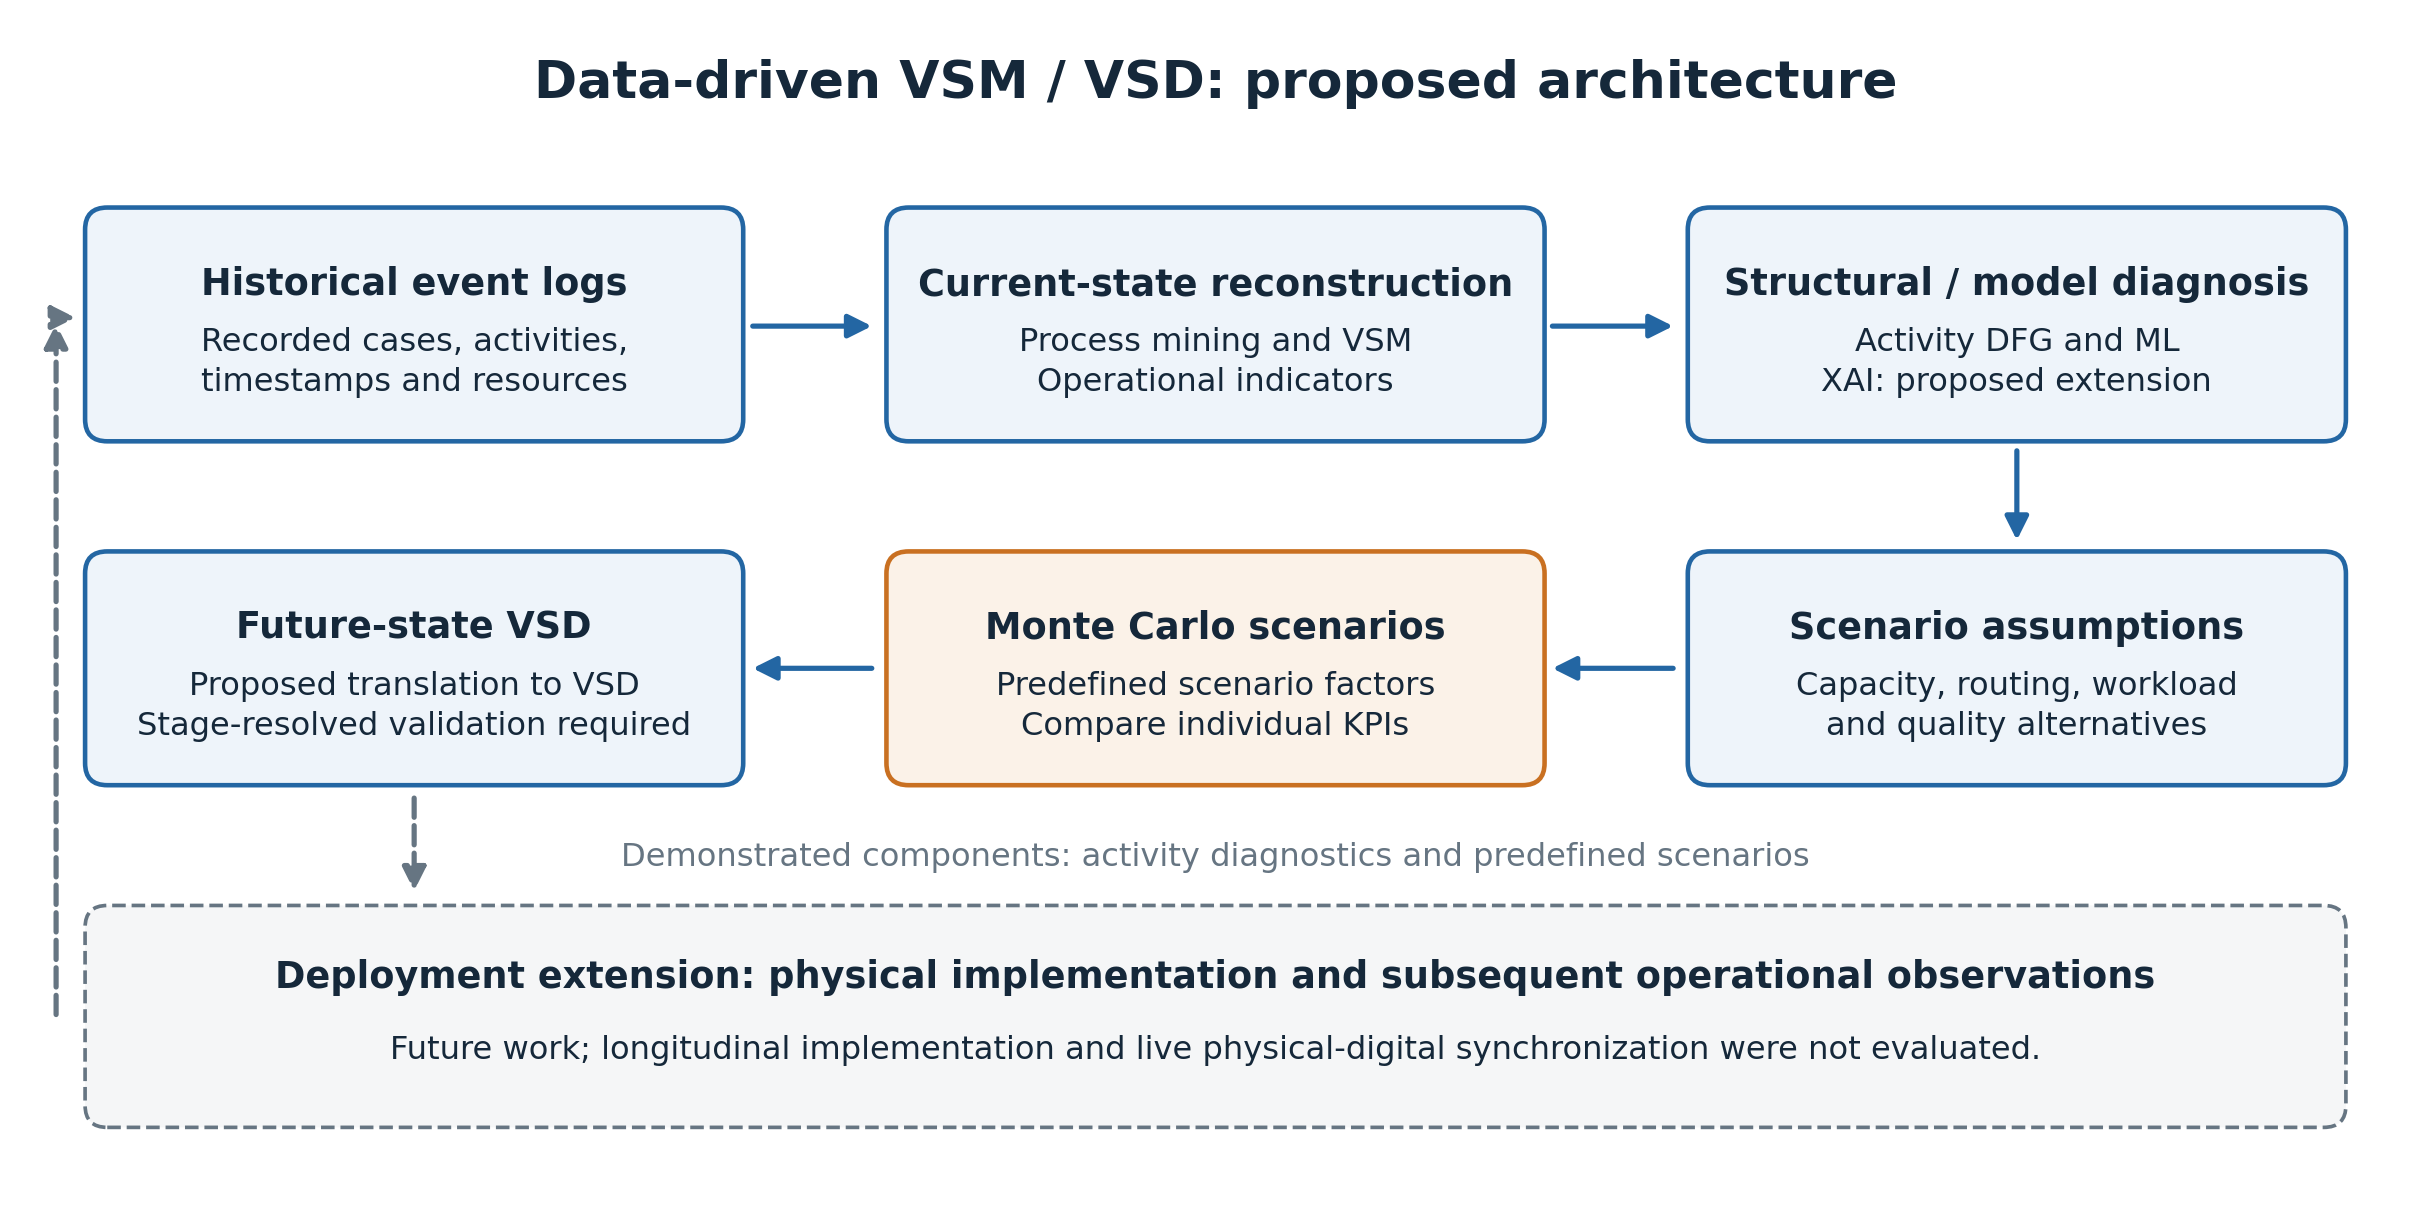
\includegraphics[width=\textwidth]{framework_architecture.png}
\caption{Research architecture and evidence boundary of the VSM/VSD framework. Historical event logs support reconstruction and diagnosis, candidate interventions are evaluated through offline MCS, and the selected configuration is represented as a future-state design. Dashed connections indicate proposed physical implementation and subsequent operational feedback, which were not evaluated. No live physical--digital synchronization is implied.}
\label{fig:framework_architecture}
\end{figure*}

Operational and network-derived features are then integrated into
Explainable Machine Learning models to identify undesirable process outcomes
and characterize the factors associated with them. Importantly, these
diagnostic outputs are not treated as the final result of the analysis.
Instead, they provide evidence for defining candidate interventions
\(\Omega_t\). The simulation model subsequently evaluates the expected
system-level consequences of these alternatives under controlled simulation
conditions.

Finally, the simulation outcomes associated with favorable candidate
configurations are translated into a future-state Value Stream Design
\(VSM_{f,t}\). The analytical sequence connects operational records, current-state reconstruction, diagnosis, intervention definition, offline evaluation, and future-state design. Physical implementation and subsequent feedback are distinguished from the evaluated analytical workflow in Figure~\ref{fig:framework_architecture}.

\subsection{Event Log Modeling and Process Mining}

The first stage of the proposed framework transforms raw operational records into structured event logs suitable for Process Mining analysis. Event logs constitute the primary data source from which process behavior, execution patterns, and performance indicators are extracted.

Let

\[
L=\{e_1,e_2,\ldots,e_n\}
\]

denote an event log composed of events generated during process execution. Each event is represented as

\[
e_i=(c_i,a_i,r_i,t_i,x_i),
\]

where \(c_i\) is the case identifier, \(a_i\) the executed activity, \(r_i\) the associated resource, \(t_i\) the timestamp, and \(x_i\) a vector of optional operational attributes.

To ensure compatibility across heterogeneous data sources, all datasets were transformed into a standardized event-log structure containing the attributes shown in Table~\ref{tab:event_schema}.

\begin{table*}[t]
\caption{
Standardized event-log schema adopted across all datasets to ensure consistent process mining, machine learning, simulation model calibration, and network-analysis workflows.
}
\label{tab:event_schema}
\centering
\begin{tabularx}{\linewidth}{p{3cm}X}
\toprule
\textbf{Attribute} & \textbf{Description} \\
\midrule

\texttt{case\_id}
&
Unique identifier of the process instance (case).
\\

\texttt{activity}
&
Name of the executed process activity.
\\

\texttt{resource}
&
Resource, operator, or machine responsible for the activity.
\\

\texttt{timestamp}
&
Execution timestamp associated with the event.
\\

\texttt{cycle\_time}
&
Processing time required to complete the activity.
\\

\texttt{waiting\_time}
&
Queueing or idle time elapsed before activity execution.
\\

\texttt{wip}
&
Work-in-process level observed at the event occurrence.
\\

\texttt{defect\_flag}
&
Binary indicator identifying defect occurrence.
\\

\texttt{rework\_flag}
&
Binary indicator identifying rework occurrence.
\\

\bottomrule
\end{tabularx}
\end{table*}

After preprocessing, Process Mining techniques were applied to discover process structures and extract operational indicators. Directly-Follows Graphs (DFGs) were employed to identify activity transitions and execution frequencies.

The process structure is represented as

\[
P=(A,E),
\]

where \(A\) denotes the set of activities and

\[
E \subseteq A \times A
\]

represents the set of directly-following relationships identified from the event log.

For each transition \((a_i,a_j)\), the execution frequency is computed as

\[
w_{ij}
=
\sum_{c\in C}
I(a_i \rightarrow a_j),
\]

where \(I(\cdot)\) is an indicator function equal to one when the transition occurs within a process instance and zero otherwise.

The discovered process model enables the estimation of key operational indicators required for Value Stream Mapping, including average cycle time, waiting time, throughput, defect rate, and rework frequency.

For an activity \(a\), the average cycle time is defined as

\[
CT(a)
=
\frac{1}{N_a}
\sum_{k=1}^{N_a}
ct_k,
\]

where \(N_a\) denotes the number of executions of activity \(a\).

Similarly, the average waiting time is computed as

\[
WT(a)
=
\frac{1}{N_a}
\sum_{k=1}^{N_a}
wt_k.
\]

These metrics constitute the quantitative foundation for the automatic generation of current-state Value Stream Maps described in the next section.


The real-log bottleneck classification label is an operational activity-level proxy. Mean cycle and waiting times are estimated per activity from training rows. An activity is flagged when either mean is at or above the corresponding training-activity 90th percentile. The label is joined to later rows by activity identity; cycle and waiting time are excluded from the bottleneck predictors. Thus, centralities can predict this label by acting as activity signatures even though betweenness does not define the target.

For delay classification, the label indicates a waiting-time proxy at or above its training-row 90th percentile; waiting time itself is excluded from the predictors. Rework classification reads the prepared binary rework flag. These are current-log diagnostic labels rather than independently observed future operational outcomes.

\subsection{Automated Current-State Value Stream Mapping}

The process model obtained through Process Mining is subsequently transformed into a current-state VSM through the automatic aggregation of operational metrics extracted from the event log. Unlike traditional VSM approaches that rely on manual observation and expert estimation, the proposed method generates quantitative value stream representations directly from process execution data.

Let

\[
P=(A,E)
\]

be the process model discovered from the event log, where \(A\) represents the set of activities and \(E\) the set of directly-following relationships. Each activity \(a \in A\) is associated with a set of operational indicators estimated during the Process Mining stage.

At activity level, mean recorded WIP is the arithmetic mean of the event-level WIP observations. Defect and rework proportions divide the respective flagged execution counts by the number of executions. These event-weighted summaries should be distinguished from time-average inventory and case-level quality rates.

To preserve compatibility with traditional Value Stream Mapping practices, activities discovered through Process Mining are grouped into value-stream stages using a predefined aggregation scheme. The mapping function

\[
\phi : A \rightarrow M
\]

assigns each low-level process activity \(a \in A\) to exactly one macro-process \(m \in M\), such that

\[
A_m = \{a \in A : \phi(a)=m\}.
\]

The aggregation scheme may be defined using domain knowledge, organizational process models, or existing production-routing structures. This aggregation preserves the hierarchical structure commonly employed in traditional Value Stream Mapping while enabling quantitative indicator estimation directly from event logs.

For each macro-process \(m \in M\), the corresponding indicators are calculated as

\[
CT_m
=
\frac{1}{|A_m|}
\sum_{a\in A_m}
CT(a),
\]

\[
WT_m
=
\frac{1}{|A_m|}
\sum_{a\in A_m}
WT(a),
\]

\[
WIP_m
=
\frac{1}{|A_m|}
\sum_{a\in A_m}
WIP(a),
\]

\[
DR_m
=
\frac{1}{|A_m|}
\sum_{a\in A_m}
DR(a),
\]

and

\[
RR_m
=
\frac{1}{|A_m|}
\sum_{a\in A_m}
RR(a).
\]

The resulting metrics are incorporated into an automatically generated Current-State Value Stream Map represented as

\[
VSM_c=(M,F,K),
\]

where \(M\) denotes the set of value stream stages, \(F\) the material and information flows connecting them, and \(K\) the associated operational indicators.

At the global process level, Lead Time is estimated as

\[
LT
=
\sum_{m\in M}
(CT_m+WT_m),
\]

while the Value-Added Ratio is computed as

\[
VAR
=
\frac{
\sum_{m\in M} CT_m
}{
\sum_{m\in M}(CT_m+WT_m)
}.
\]

The additive lead-time representation corresponds to a sequential-stage approximation. Branches, repeated visits, and concurrency require interpretation against the corresponding case boundaries. Likewise, the processing-time fraction is a time-decomposition indicator; calling it value added requires domain knowledge because processing, inspection, and repetition are not automatically value-creating activities.

The automatically generated VSM provides a quantitative representation of process performance and serves as the foundation for subsequent network analysis, predictive modeling, and offline Monte Carlo simulation.

\subsection{Complex Network Modeling and Feature Engineering}
\label{subsec:complex_networks}

Although Process Mining and Value Stream Mapping provide valuable process-level insights, they are often insufficient for capturing the structural dependencies and interaction patterns that emerge among activities, resources, and value flows. To address this limitation, the proposed framework incorporates CNA to model the operational system from multiple complementary perspectives.

The architecture can accommodate three complementary graph representations. The supplied experiments construct the activity graph; resource and value-flow networks remain proposed extensions:

\[
\mathcal{G}
=
\{
G_A,
G_R,
G_V
\},
\]

where \(G_A\) represents the Activity Network, \(G_R\) the Resource Network, and \(G_V\) the Value-Flow Network. The Activity Network captures directly-following relationships among process activities, the Resource Network models interactions among operators, machines, and organizational resources, and the Value-Flow Network represents material, information, and product transfers across value-stream stages.

To characterize the implemented activity graph, standard graph-theoretic indicators were computed, including degree, betweenness, closeness, and eigenvector centrality. These metrics quantify node connectivity, intermediary influence, accessibility, and structural importance, respectively. In addition, network density was calculated to characterize the overall connectivity of the process structure and provide a global indicator of interaction complexity.

The implemented centralities use an unweighted undirected projection of the activity DFG; descriptive density is computed on the directed graph. Self-loops are retained by the supplied graph construction, so degree normalization follows the library convention and may exceed one. Simultaneous timestamps do not establish a unique causal ordering of activities.

Detailed mathematical definitions of these metrics can be found in the complex-network literature \cite{newman2018networks,freeman1978centrality}.

The resulting network-derived attributes were integrated with operational indicators extracted from Process Mining and Value Stream Mapping to create a unified feature space:

\[
\mathbf{X}
=
\{
\mathbf{X}_{PM},
\mathbf{X}_{VSM},
\mathbf{X}_{CN}
\},
\]

where \(\mathbf{X}_{PM}\), \(\mathbf{X}_{VSM}\), and \(\mathbf{X}_{CN}\) denote Process Mining, Value Stream Mapping, and Complex Network features, respectively.

The resulting feature matrix combines operational and structural information, enabling the identification of critical activities, process bottlenecks, and interaction patterns that may not be observable through conventional process indicators alone. Activity-level descriptors are used by the implemented classification layer. Explainability and the additional network perspectives are proposed extensions.

\subsection{Classification and Proposed Explainability Layer}
\label{subsec:xai_ml}

The executed classification layer uses Random Forest and XGBoost with fixed hyperparameters. Its inputs combine the available operational attributes with activity-level centralities. The comparisons concern the prepared defect, repetition/rework, delay, and operational-bottleneck proxy labels, depending on the dataset. Accuracy, precision, recall, F1-score, and ROC-AUC summarize held-out classification when both relevant classes are present.

The architecture can be extended with SHAP explanations to characterize feature associations. However, the supplied scripts do not execute a SHAP layer, and no explanation-derived intervention effect is estimated in the reported experiments. Interpretability evidence added in the synthetic audit instead comes from a direct activity-majority rule and a comparison with activity-only classification.

Algorithm~\ref{alg:vsm_generation} separates the implemented diagnostic steps from optional architectural extensions. A descriptive full-log activity graph may be used for visualization; classification features require an explicitly training-only graph. Candidate-intervention factors in the supplied scenario sampler are specified independently of these outputs.

\begin{algorithm}[!t]
\caption{Implemented diagnostic steps and proposed extensions}
\label{alg:vsm_generation}
\textbf{Input:} Event log \(L\).\\
\textbf{Output:} Process indicators, activity descriptors, and classification results.
\begin{enumerate}
\item Validate the event schema and document measured versus proxy quantities.
\item Construct a descriptive activity DFG and summarize process indicators.
\item Partition classification rows chronologically; construct activity-network features from training rows only for the audited comparison.
\item Fit matched operational-only and network-augmented classifiers with the stated task-specific exclusions.
\item Compare with activity-only rules, save held-out predictions, and interpret target/feature availability.
\item As deployment extensions, add independent explanations, resource/value-flow perspectives, and validated intervention linkage.
\end{enumerate}
\end{algorithm}

\subsection{Offline Simulation-Based Future-State Design}
\label{subsec:digital_twin_future_state}

The numerical demonstration uses an offline Monte Carlo scenario sampler implemented in NumPy. For each of six predefined factor sets, it samples 500 independent orders per replication and performs 30 replications. It does not execute a discrete-event calendar, shared resources, or a physical--digital synchronization mechanism.

\begin{table*}[t]
\caption{Predefined factors used by the original scenario sampler. Scenario names identify the assumed analysis-support level; factors are input assumptions, not effects estimated from PM, ML, XAI, or CNA outputs.}
\label{tab:scenario_factors}
\centering\small
\begin{tabular}{lrrrr}
\toprule
Scenario & Cycle factor & Waiting factor & Defect factor & Additional gain\\
\midrule
G0 & 1.00 & 1.00 & 1.00 & 0.00\\
G1 & 0.98 & 0.92 & 0.97 & 0.00\\
G2 & 0.96 & 0.85 & 0.95 & 0.00\\
G3 & 0.92 & 0.78 & 0.88 & 0.00\\
G4 & 0.88 & 0.68 & 0.82 & 0.02\\
G5 & 0.84 & 0.58 & 0.72 & 0.06\\
\bottomrule
\end{tabular}
\end{table*}

Order processing time is the sum of truncated normal draws at the seven route stations, multiplied by the cycle factor. Waiting is sampled from gamma distributions and multiplied by the waiting factor. Station defect indicators use the specified probabilities multiplied by the defect factor. Conditional rework adds a sampled duration, and the resulting lead time is multiplied by one minus the additional-gain factor. The parameter named \texttt{network\_gain} in the original script is this additional assumption; it is not a gain estimated from network structure.

The reported WIP quantity is a workload proxy: a nonnegative normal draw centered at sampled waiting time divided by eight, multiplied by one minus the additional gain. The throughput proxy divides the 500 orders by a constructed calendar horizon, equal to 500 times 7.5 minutes times the waiting factor plus mean order lead time. These conventions produce reproducible scenario indicators, not inventory or completion counts from a resource-constrained queueing simulation.

Each replication uses seed \(1000+r\), where \(r=1,\ldots,30\), for every scenario. Within each scenario the replications vary independently; across scenarios the replication identifier defines a shared initial-seed block. Random draw paths can diverge because scenario-dependent quality outcomes affect conditional sampling.

The scenario performance vector contains mean sampled lead time, the calendar-based throughput proxy, the workload proxy, mean station defect proportion, and the proportion of sampled orders assigned rework. The quality measures have distinct denominators and should not be interpreted as the same event-level rate.

The performance of each configuration is evaluated relative to the baseline
configuration \(G_0\). For an indicator to be minimized,
\(k\in\{LT,WIP,DR,RR\}\), the relative improvement is computed as

\[
I_k^{(j)}
=
\frac{
k_{G_0}-k_{G_j}
}{
k_{G_0}
}
\times 100.
\]

For throughput, for which larger values are preferred, the improvement is
computed as

\[
I_{TH}^{(j)}
=
\frac{
TH_{G_j}-TH_{G_0}
}{
TH_{G_0}
}
\times 100.
\]

This formulation allows the incremental performance associated with
progressively enriched configurations to be quantified without aggregating
heterogeneous KPIs into a single optimization objective.
A configuration is considered operationally preferable when it improves
throughput while simultaneously reducing lead time, work-in-process, defect
rate, and rework rate.

The proposed framework can map an evaluated intervention back to a future-state representation. A stage-resolved deployment would require stage-specific simulated outputs, routing and resource effects, and domain-validated value indicators. The supplied sampler reports aggregate scenario KPIs; it does not automatically produce a validated stage-level future-state map. The numerical results therefore illustrate scenario comparison within the broader proposed architecture.

\subsection{Closed-Loop Data-Driven VSM/VSD Framework}
\label{subsec:closed_loop_framework}

Building upon the problem formulation introduced in
Section~\ref{subsec:problem_formulation}, the complete framework establishes
a traceable analytical path from operational event data to evidence-based
Future-State Value Stream Design. Rather than representing the framework as
a sequence of independent technologies, its analytical stages correspond to
the main decision-support functions required to transform observed process
behavior into an evaluated redesign alternative.

The available log \(L_t\) supports a current-state map \(VSM_{c,t}\), diagnostic evidence, a set of candidate configurations \(\Omega_t\), their simulation-based assessment, and the future-state representation \(VSM_{f,t}\).

The proposed architecture organizes four intended decision-support functions; the numerical implementation evaluates only the components identified below.
First, operational event data are transformed into a quantitative
current-state representation through Process Mining and automated VSM
generation. Second, operational indicators, Complex Network Analysis, and
Explainable Machine Learning provide complementary evidence for identifying
process criticalities and their associated factors. Third, this diagnostic
evidence supports the definition of candidate interventions, whose expected
system-level consequences are evaluated through offline Monte Carlo simulation.
Finally, the simulation outputs are mapped back to the value-stream
representation to construct and assess the corresponding future-state design.

Candidate configurations are compared with the current state for each KPI separately: lower lead time, WIP, defect rate, and rework rate and higher throughput are favorable. Simultaneous improvement is a useful comparison criterion, not a mandatory constraint on every candidate. When indicators conflict, the individual changes remain visible to decision makers.

Algorithm~\ref{alg:closed_loop} summarizes the proposed architecture. The executed activity-network, diagnostic-classification, and scenario components are distinguished from deployment extensions in the accompanying text.

\begin{algorithm}[!t]
\caption{Proposed VSM/VSD architecture and deployment extensions}
\label{alg:closed_loop}
\textbf{Input:} Operational event log \(L_t\).\\
\textbf{Output:} Evaluated Future-State Value Stream Design \(VSM_{f,t}\).
\begin{enumerate}
\item Reconstruct observed process behavior from \(L_t\), generate the
Current-State VSM \(VSM_{c,t}\), and extract operational indicators.
\item Construct the activity network and compute its structural indicators; extend to resource and value-flow networks when corresponding data and validation are available.
\item Fit diagnostic classifiers with operational and training-only network features to construct evidence \(\mathcal{D}_t\); add an explanation layer as a deployment extension.
\item Specify candidate configurations \(\Omega_t\) and document their parameter provenance. In the evaluated sampler, scenario factors are predefined rather than estimated from diagnostic models.
\item For each \(S_i\in\Omega_t\), perform repeated simulations, estimate
\(\mathbf{K}_{f}^{(i)}\), and compare it with \(\mathbf{K}_{c}\).
\item Identify favorable configurations, map the selected configuration to
\(VSM_{f,t}\), and return \(VSM_{f,t}\).
\end{enumerate}
\end{algorithm}

The architecture does not require online connectivity between an operational system and a simulation model. In this study, the synthetic route inputs and predefined scenario factors parameterize the offline sampler; outputs from the diagnostic classifiers do not determine those factors. Automatic explanation-driven intervention selection and a validated stage-resolved future-state map remain deployment extensions.

In an industrial deployment, an evaluated future-state design could be implemented and a subsequent observation period could provide a new log for another analytical cycle. This recurrent physical feedback is a deployment mechanism rather than an experimentally evaluated component of the present study.

%============================================================
% 4. EXPERIMENTAL DESIGN
% ============================================================

\section{Experimental Design}
\label{sec:experimental_design}

This section describes the numerical demonstration and diagnostic checks supporting the proposed VSM/VSD architecture. The evaluation comprises predefined simulated operational changes, prepared-label classification, and activity-network summaries. Cross-domain comparisons assess those analytical components; the scenario comparison quantifies responses to assumed factors rather than effects of progressively activating fitted modules.

\subsection{Experimental Objectives and Datasets}
\label{subsec:experimental_objectives}

The evaluation examines diagnostic behavior across the selected prepared benchmarks and operational responses within the synthetic sampler. It compares operational-feature, network-augmented, and activity-only classifiers and documents the predefined scenario factors. It does not estimate the causal effect of implementing the full architecture relative to conventional VSM in a physical plant.

The experiments were conducted using the datasets described in Section~\ref{subsec:datasets}, comprising one synthetic manufacturing event log and three real-world event logs. The synthetic manufacturing dataset was employed for controlled experimentation, simulation parameterization, simulation-based evaluation of cumulative framework configurations, and statistical scenario comparison under reproducible operating conditions. The real-world event logs were subsequently used to assess analytical applicability of the proposed framework across heterogeneous operational domains, including business processes, procurement workflows, and manufacturing environments affected by data-quality issues.

Three complementary dimensions were considered throughout the experimental evaluation.

\begin{itemize}

\item \textbf{Operational scenario evaluation} summarizes lead time, workload and throughput proxies, defect rate, and rework rate under predefined factors. These changes characterize the sampler and do not establish observed intervention benefits.

\item \textbf{Diagnostic classification} compares operational-feature and network-augmented models on the prepared delay, bottleneck, and rework labels. Activity-only controls and target-definition checks bound the interpretation; these comparisons do not establish prospective prediction.

\item \textbf{Structural evaluation} summarizes activity-transition connectivity and centrality. Resource dependencies and value-flow graphs are proposed extensions, not measured network layers in the supplied experiments.

\end{itemize}

Across domains, the shared numerical protocol uses the prepared event schema, process summaries, activity-network construction, and diagnostic classification. The original and corrected executions are documented separately. Explainability layers and resource/value-flow networks are architectural extensions. Operational scenario changes are evaluated only within the synthetic manufacturing sampler; the real-world logs do not establish manufacturing intervention gains.

\subsection{Scenario Comparison Design}
\label{subsec:ablation}

The original numerical comparison names six scenarios after increasing levels of analytical support. In the executable sampler, those names select the fixed parameter factors in Table~\ref{tab:scenario_factors}. They do not switch fitted analytical components on or off. The comparison is therefore interpreted as a structured scenario demonstration, not an executed component-ablation study. Individual or cumulative causal benefits of analytical modules cannot be identified from these factors.

The cumulative experimental configurations considered in this study are summarized in Table~\ref{tab:ablation_groups}.

\begin{table*}[t]
\caption{
Scenario labels retained from the original comparison. The executable sampler uses their predefined factors; the labels do not demonstrate activation of fitted analytical modules.
}
\label{tab:ablation_groups}
\centering
\begin{tabularx}{\linewidth}{p{1.2cm}X}
\toprule
\textbf{Group} & \textbf{Description} \\
\midrule

G0 &
Baseline operational process without analytical decision-support mechanisms.
\\

G1 &
Traditional manually constructed VSM.
\\

G2 &
Automatically generated Process Mining-based Value Stream Mapping (PM-VSM).
\\

G3 &
PM-VSM enriched with Explainable Machine Learning for predictive process diagnosis.
\\

G4 &
PM-VSM combined with Explainable Machine Learning and simulation-based future-state scenario evaluation.
\\

G5 &
Complete framework integrating Process Mining, Explainable Machine Learning, offline Monte Carlo simulation, and Complex Network Analysis.
\\

\bottomrule
\end{tabularx}
\end{table*}

G0 is the reference factor set; G1--G5 represent progressively more favorable assumptions about processing, waiting, quality, and an additional multiplicative gain. The reported scenario names retain the intended conceptual association with manual VSM, PM, ML/XAI, simulation, and CNA, but the scripts do not estimate factor values from those technologies. Operational comparisons concern simulated indicators; classification comparisons are evaluated separately.

\subsection{Evaluation Metrics}
\label{subsec:metrics}

The proposed framework is evaluated from three complementary perspectives: operational performance, predictive capability, and structural process behavior. Operational indicators quantify Lean-oriented process performance, predictive metrics evaluate the effectiveness of the Explainable Machine Learning layer, and structural indicators characterize process topology through Complex Network Analysis.

Table~\ref{tab:evaluation_metrics} summarizes the metrics employed throughout the experimental evaluation.

\begin{table*}[t]
\caption{
Evaluation metrics employed to assess operational performance, predictive capability, and structural process characteristics.
}
\label{tab:evaluation_metrics}
\centering
\begin{tabularx}{\textwidth}{p{2.5cm}p{4.8cm}X}
\toprule
\textbf{Category} &
\textbf{Metrics} &
\textbf{Purpose} \\
\midrule

Operational
&
Lead time, throughput, WIP, CT, defect rate, rework rate
&
Evaluation of process efficiency, operational performance, and Lean-oriented improvement achieved through successive cumulative framework configurations.
\\

Predictive
&
Accuracy, Precision, Recall, F1-score, ROC-AUC
&
Assessment of predictive models for delay, bottleneck, and rework prediction using conventional process features and network-derived structural features.
\\

Structural
&
Degree Centrality, Betweenness Centrality, Closeness Centrality, Eigenvector Centrality, Network Density
&
Characterization of process topology and identification of structurally relevant activities, resource dependencies, and connectivity patterns through Complex Network Analysis.
\\

\bottomrule
\end{tabularx}
\end{table*}

Operational performance is evaluated on the cumulative experimental configurations (G0--G5) using the offline Monte Carlo simulation environment. Predictive performance is evaluated independently on the real-world event logs using temporal train-validation-test partitions, whereas structural analysis quantifies the additional information provided by network-derived features beyond conventional process indicators.

Because the proposed framework integrates complementary analytical components, no single metric is sufficient to characterize its overall performance. Instead, the combined use of operational, predictive, and structural metrics provides a multidimensional evaluation of the framework's capability to support current-state analysis, predictive diagnosis, simulation-based intervention assessment, and future-state Value Stream Design.

\subsection{Model Training and Simulation Protocol}
\label{subsec:training_protocol}

The experimental evaluation combines predictive modeling with simulation-based experimentation to assess complementary aspects of the proposed framework. Explainable Machine Learning is employed to identify operational criticalities from historical event logs, whereas the simulation model is used to evaluate the operational consequences of alternative future-state VSD configurations before implementation.

For the predictive experiments, real-world event logs are partitioned using a temporal train--validation--test strategy to preserve the chronological order of process executions and reduce the possibility of information leakage. The adopted partition allocates 70\% of the observations for training, 15\% for validation, and 15\% for independent testing.

Random Forest is employed as an interpretable baseline model, while XGBoost is adopted as the primary predictive algorithm because of its ability to model nonlinear relationships and complex interactions among operational and network-derived features.

To further reduce target leakage, proxy labels requiring threshold estimation are generated only after the temporal partition. In particular, thresholds used to define delay-related targets are estimated exclusively from the training subset and subsequently applied to the validation and testing partitions. Likewise, predictor variables directly involved in constructing a target variable are excluded from the corresponding predictive models. Specifically, \textit{waiting time} is excluded from delay classification. Both \textit{cycle time} and \textit{waiting time} are excluded from operational bottleneck-proxy classification. Betweenness is not used to define that target in the supplied script.

The validation subset is reserved but is not used by the supplied script for model selection. Hyperparameters are fixed, and the reported scores refer to the held-out testing rows. Fixed random seeds are employed throughout the complete predictive pipeline to facilitate experimental reproducibility.

The temporal partition and predictor exclusions address specific leakage routes, but do not establish that every network descriptor is available at a prospective decision timestamp. In particular, graph metrics can encode activity identity and structural properties associated with a proxy label. The reported experiments therefore support held-out event-log classification and diagnostic analysis under the stated representation. They are not presented as a validated forecast of future rework from partial case histories. Such a prospective task would additionally require a defined prediction timestamp and horizon, prefix-only attributes, causally available graph construction, and explicit handling of cases spanning temporal boundaries.

The scenario sampler reads the synthetic route parameters and predefined factor sets, without loading model predictions, explanations, or estimated network effects. Simulation-based evaluation is subsequently performed over the cumulative experimental configurations defined in Section~\ref{subsec:ablation}, ranging from the baseline process (G0) to the complete framework (G5).

For each scenario, 30 replications sample processing times, waiting-time proxies, and quality/rework events. The same initial seed is reused for a given replication number across scenarios; routing and shared-resource utilization are not solved by this sampler. The resulting configurations are compared using Lead Time, Throughput, Work-In-Process, Defect Rate, and Rework Rate. Mean KPI values, standard deviations, 95\% confidence intervals, and relative improvements with respect to the baseline configuration are reported.

The supplied sampler evaluates combinations of processing, waiting, quality, and additional-gain factors. Capacity and shared-resource interventions require a richer operational simulator. In the present study, however, statistical comparisons are performed across the cumulative framework configurations (G0--G5) rather than through optimization-based ranking of independently generated intervention alternatives.

Unlike the simulation experiments, the predictive evaluation on the real-world event logs does not involve repeated stochastic replications. Consequently, predictive performance is reported only for the independent testing partition, whereas measures of statistical variability, including standard deviations and 95\% confidence intervals, are reported exclusively for the offline Monte Carlo simulation experiments, where repeated replications permit statistically meaningful estimation of variability.

To quantify the contribution of Complex Network Analysis, every predictive task is executed twice. The first experiment uses only conventional process and Value Stream Mapping features, whereas the second incorporates additional network-derived structural features. Improvements observed under the second configuration quantify the additional predictive information provided by structural process analysis beyond conventional operational indicators.

\subsection{Statistical Validation and Research Hypotheses}
\label{subsec:statistical_validation}

Statistical analyses were conducted to determine whether the operational differences observed across the cumulative experimental configurations exceeded the variability introduced by stochastic simulation. Because the simulation model experiments involve repeated stochastic replications, inferential statistical analyses were performed exclusively for the simulation-based operational evaluation.

The code audit supplements the original independent-group analysis with seed-blocked comparisons. Friedman tests compare the six scenarios over 30 replication blocks. Two-sided Wilcoxon signed-rank tests compare each of G1--G5 with G0, with Holm adjustment across the five baseline comparisons within each KPI. Relative-change intervals use 10,000 paired-block bootstrap resamples with seed 20261024; the statistic is a ratio of scenario means. These intervals characterize stochastic variation conditional on the chosen sampler and factors. They do not include industrial-calibration uncertainty. No global multiplicity adjustment across all KPI families is asserted.

Unlike the simulation experiments, predictive evaluation on the real-world event logs does not involve repeated stochastic replications. Consequently, predictive performance is assessed through out-of-sample evaluation on the held-out temporal-row testing partition using Accuracy, Precision, Recall, F1-score, and ROC-AUC. Improvements associated with Complex Network Analysis are quantified by comparing predictive models trained with conventional process features against models additionally incorporating network-derived structural features.

The experimental evaluation addresses the following research hypotheses.

\begin{itemize}

\item \textbf{H1.} The predefined scenario configurations differ in their model-generated indicators relative to the baseline, as measured by Lead Time, Throughput, Work-In-Process, Defect Rate, and Rework Rate.

\item \textbf{H2.} Incorporating network-derived structural features improves the predictive performance of Machine Learning models for delay, bottleneck, and rework prediction compared with models based exclusively on conventional process and Value Stream Mapping features.

\item \textbf{H3.} The predefined synthetic scenarios exhibit simultaneous favorable changes in multiple model-defined indicators; this is a within-model proposition rather than evidence of causal module integration.

\end{itemize}

For the simulation experiments, the null hypothesis assumes that no statistically significant differences exist among the evaluated cumulative configurations, whereas the alternative hypothesis assumes that at least one configuration produces significantly different operational performance. For the predictive experiments, H2 is evaluated through direct comparison of out-of-sample predictive performance obtained with and without network-derived structural features.

It is important to emphasize that the cumulative experimental design evaluates progressively enriched analytical workflows rather than isolated analytical components. Consequently, statistically significant differences among cumulative configurations should be interpreted as evidence of conditional scenario differences and not as independent causal estimates of the individual contribution of each analytical capability.


\subsection{Threats to Validity}
\label{subsec:threats_to_validity}

As with any empirical study integrating multiple analytical methodologies, several factors may influence the validity and generalizability of the obtained results. The principal threats to validity considered in this study are summarized below.

\textbf{Internal validity.}
The cumulative simulation configurations share a common model environment and evaluation indicators. The classification comparisons use the stated temporal partitioning and matched operational-only and CNA-augmented feature sets. Fixed random seeds were employed throughout the predictive and simulation experiments to reduce variability introduced by stochastic model training and simulation execution. Furthermore, proxy labels requiring threshold estimation were generated exclusively from the training partition, and predictor variables directly involved in defining a target variable were excluded from the corresponding predictive models in order to reduce target leakage.

\textbf{Construct validity.}
Operational, predictive, and structural evaluation metrics were selected according to widely adopted practices in Lean Manufacturing, Process Mining, Machine Learning, and Complex Network Analysis. Nevertheless, some proxy variables, including delay, bottleneck, and rework indicators, are operational approximations derived from event-log information rather than directly observed organizational labels. Consequently, their interpretation depends on the quality and granularity of the available process data. Structural-proxy classification and event repetition must not be equated with independently observed future bottlenecks or corrective work. High F1 on these proxies does not establish prospective prediction performance.

\textbf{External validity.}
The full operational comparison was conducted in a controlled synthetic manufacturing environment. Its improvement magnitudes are conditional on the modeled distributions, routing, resource capacities, and intervention settings. The administrative BPI benchmarks assess analytical components; they do not validate physical shop-floor outcomes. Longitudinal industrial studies with implemented interventions are required to assess transfer, including under breakdowns, changing demand, noisy records, and exceptional routing.

\textbf{Model and data validity.}
The predictive performance of the proposed framework depends on the quality, completeness, and representativeness of the underlying event logs. Likewise, offline Monte Carlo simulations necessarily rely on calibration assumptions regarding processing times, waiting times, routing behavior, resource utilization, and operational variability. Standardized preparation, multiple models, and repeated simulation runs address some sources of variability. Replication confidence intervals quantify variation conditional on the simulator; they do not establish fidelity to a physical factory or uncertainty about model assumptions.

\textbf{Methodological validity.}
The predefined scenario design adopted in this study evaluates progressively enriched analytical workflows rather than isolated analytical components. Consequently, statistically significant differences among cumulative configurations should be interpreted as conditional scenario differences rather than independent causal estimates of each analytical capability. In addition, although the proposed framework defines a closed analytical loop connecting Process Mining, Explainable Machine Learning, Complex Network Analysis, offline Monte Carlo simulation, and Future-State Value Stream Design, the present study evaluates this workflow in an offline analytical setting. Continuous online deployment, recurrent simulation model recalibration, and streaming event-log processing remain important directions for future research.

Despite these limitations, the combination of controlled synthetic experimentation, heterogeneous real-world datasets, temporal validation protocols, statistical analysis, and cumulative framework evaluation provides a rigorous and reproducible basis for assessing the effectiveness of the proposed data-driven VSM/VSD framework.

\section{Results}
\label{sec:results}

This section presents the experimental evaluation of the proposed data-driven VSM/VSD framework. The results are organized into four complementary parts. First, the framework is evaluated under controlled conditions using the synthetic manufacturing event log, allowing quantitative analysis of the cumulative framework configurations through offline Monte Carlo simulation. Second, the analytical components are assessed on three heterogeneous real-world event logs for classification and structural description across domains. Third, the scenario comparison quantifies the incremental operational improvements obtained as additional analytical capabilities are progressively incorporated into the framework. Finally, statistical analyses determine whether the observed operational improvements exceed the variability introduced by stochastic simulation.

\subsection{Experimental Results on the Synthetic Manufacturing Event Log}
\label{subsec:synthetic_results}

The proposed data-driven VSM/VSD framework was first evaluated using a
synthetic manufacturing event log designed to represent controlled production
flows, waiting times, rework activities, quality events, and resource
interactions under controlled experimental conditions. Six analytical
configurations were considered, ranging from a baseline representation of
the process to the complete framework integrating PM,
automated VSM, ML, offline MCS, and CNA. The main results are
summarized in Figure~\ref{fig:synthetic_results}.

\begin{figure*}[t]
\centering
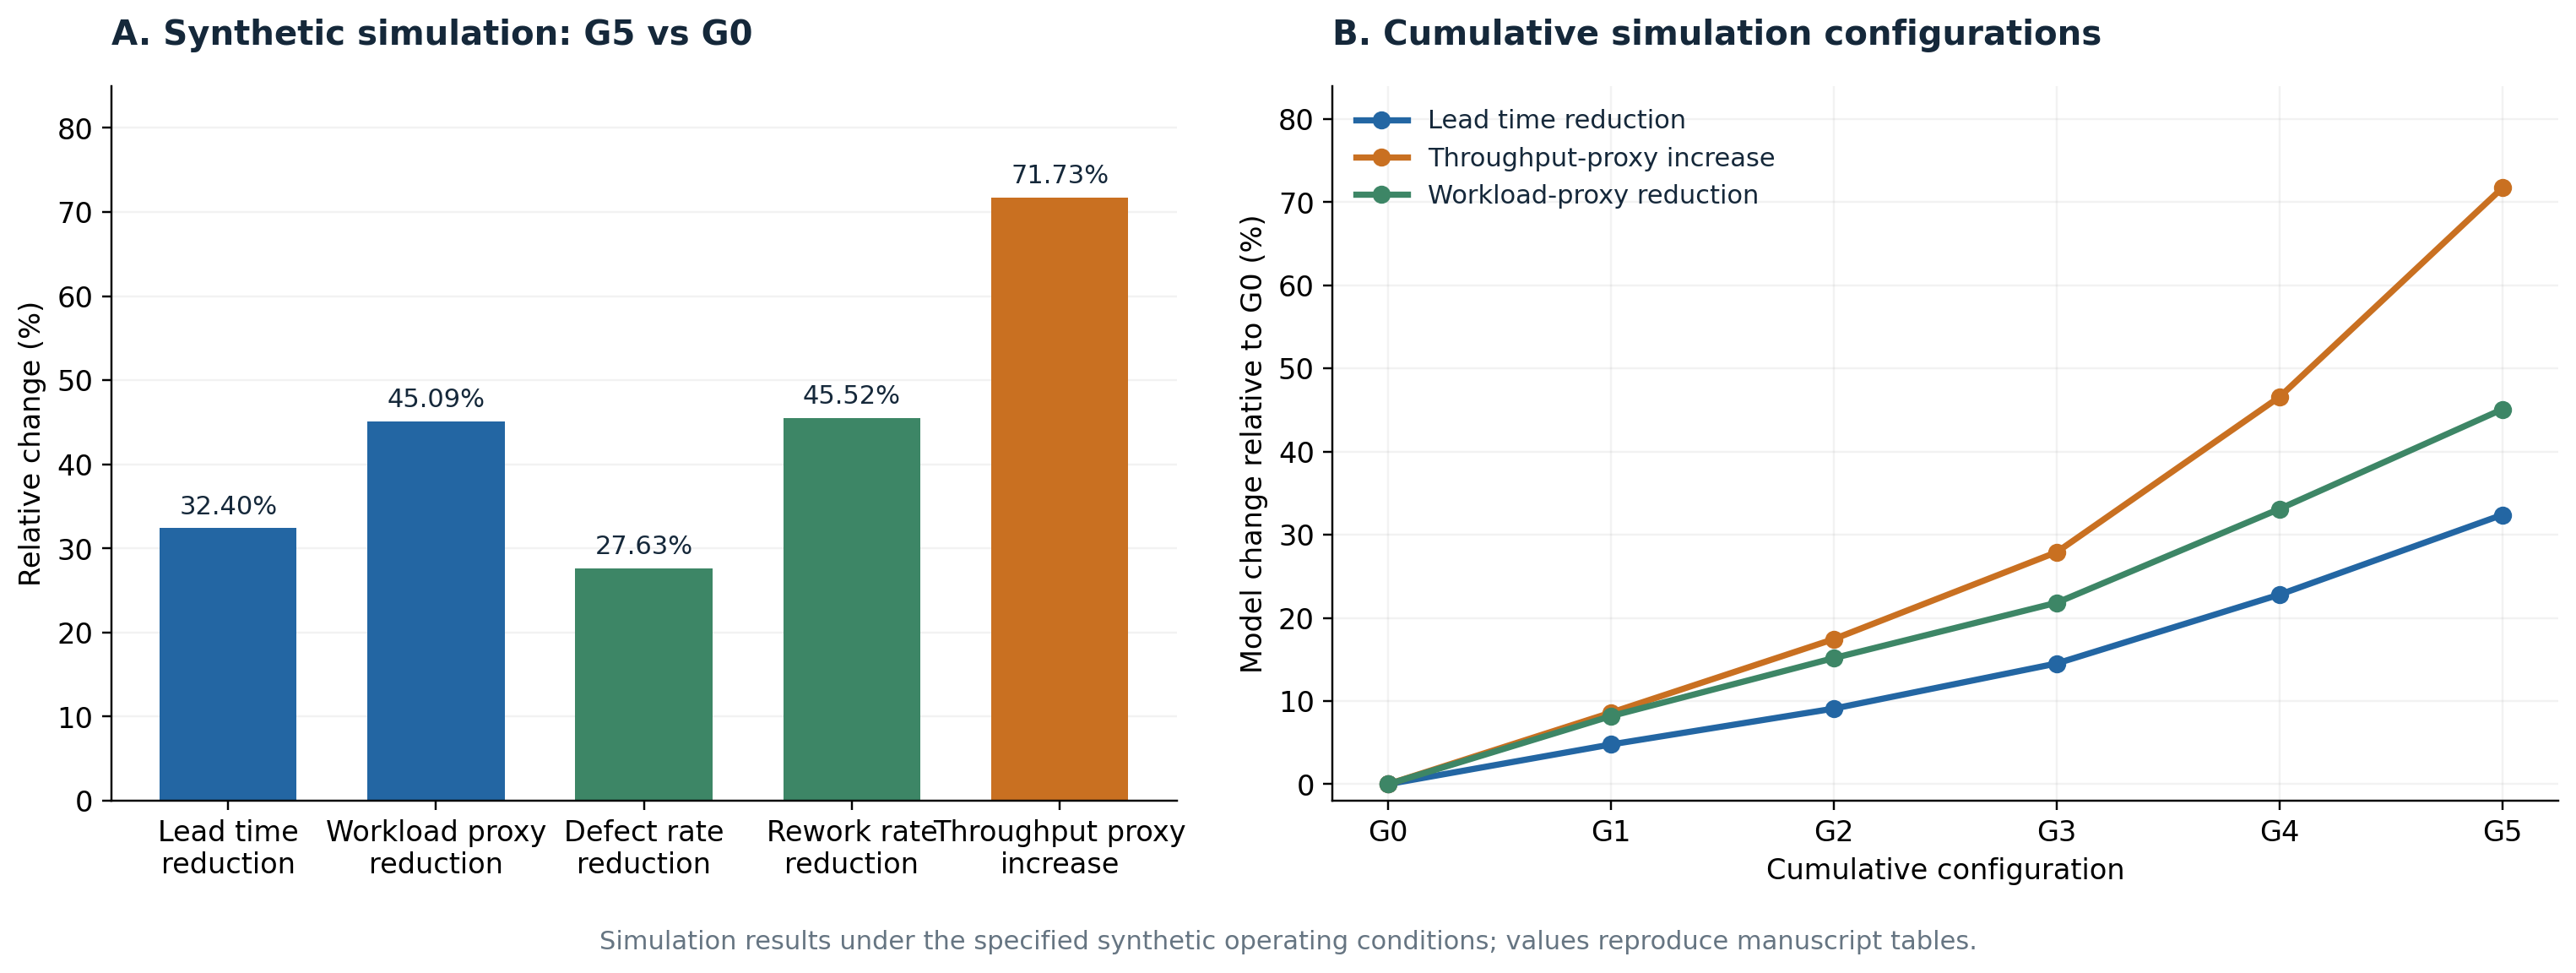
\includegraphics[width=\textwidth]{paper_synthetic_results_final_dashboard.png}
\caption{Synthetic manufacturing simulation results. (A) G5 relative KPI changes versus G0, using the values in Table~\ref{tab:synthetic_improvements}. (B) Cumulative lead-time, throughput, and WIP changes from Table~\ref{tab:ablation_results}. All changes concern simulated scenarios, not physical factory measurements.}
\label{fig:synthetic_results}
\end{figure*}

Figure~\ref{fig:synthetic_results}A summarizes the simulated G5 changes relative to G0. As reported in Table~\ref{tab:synthetic_improvements}, lead time, WIP, defect rate, and rework rate decrease, while throughput increases. These values describe the selected synthetic operating conditions and intervention configurations.

\begin{table*}[t]
\caption{
Model responses under the predefined G5 factor set relative to G0. Workload and throughput quantities follow the proxy conventions of the scenario sampler.
}
\label{tab:synthetic_improvements}
\centering
\begin{tabular}{lc}
\toprule
\textbf{Metric} & \textbf{Improvement (\%)} \\
\midrule
Lead Time Reduction & 32.40 \\
Work-in-Process Reduction & 45.09 \\
Defect Rate Reduction & 27.63 \\
Rework Rate Reduction & 45.52 \\
Throughput Increase & 71.73 \\
\bottomrule
\end{tabular}
\end{table*}

Figure~\ref{fig:synthetic_results}B shows progressively larger simulated changes across G0--G5. The comparison is cumulative: analytical capabilities support intervention choices whose operational effects are evaluated in the simulator. Adding an analytical module does not by itself alter physical process behavior, and the design does not isolate independent causal effects of individual modules.

The synthetic setting enables controlled comparison, but it cannot reproduce every source of variability in industrial production. The exact magnitudes therefore remain scenario specific. Manufacturing deployment would require calibration and independent checking against plant observations, followed by measurements of implemented interventions under documented operating conditions.

\subsubsection{Code-Level Audit of the Synthetic Classification Task}
\label{subsec:synthetic_code_audit}

The delivered synthetic data contain 8,532 events from 1,200 cases and eight observed activities. The flag \texttt{rework\_flag} equals the indicator of the activity \texttt{Rework} in every row. In the chronological test partition, 21 of 1,280 rows are positive. A rule learned only from training rows that predicts each activity's majority label attains F1 = 1.0000, as do an activity-only Random Forest and a Random Forest using training-only centralities. Their confusion matrix is TN = 1,259, FP = 0, FN = 0, TP = 21.

\begin{table*}[t]
\caption{Executed synthetic rework audit. All rows use the same 70/15/15 temporal row split; graph features and activity rules are fitted on training rows only. These are diagnostic-label results, not prospective forecasts.}
\label{tab:synthetic_audit}
\centering\small
\begin{tabular}{lr}
\toprule
Condition & Test F1\\
\midrule
Training-only activity-majority rule & 1.0000\\
Random Forest, operational variables & 0.2500\\
Random Forest, training-only network descriptors & 1.0000\\
Random Forest, operational and training-only network descriptors & 1.0000\\
Random Forest, activity one-hot representation & 1.0000\\
\bottomrule
\end{tabular}
\end{table*}

The four centralities give distinct signatures to all eight activities. Although the original synthetic script loads full-log centralities before splitting, reconstructing the graph using training rows alone produces numerically identical values in this dataset. The audit therefore identifies activity/label reconstruction as a sufficient explanation of its perfect rework F1; it does not attribute the score to a measured difference between full-log and training-only centralities. This experiment does not establish the BPI2017 mechanism by itself; the separate real-log audit establishes the association in its prepared rows.

The synthetic delay flag also equals \texttt{waiting\_time\_min > 15} in every row, and the original synthetic model includes that same waiting variable. Its near-perfect delay score consequently reconstructs the generating rule. This is not evidence of anticipating delays before the relevant information exists. The original row split shares two cases between training and validation and three between validation and test; training and test share no cases. Two pre-test events finish at or after the test start. A prospective design would need an explicit observation cutoff and case-boundary policy rather than relying on row ordering alone.

\subsection{Results on Real-World Event Logs}
\label{subsec:real_results}

To evaluate the generalizability of the proposed framework beyond controlled
experimentation, the methodology was applied to three heterogeneous
real-world event logs exhibiting different operational characteristics,
process complexity, and organizational contexts: BPI2017, BPI2019, and the
Data Quality Issues (DQI) dataset. Collectively, these datasets provide a
challenging evaluation environment that includes large-scale business
processes, procurement workflows, and manufacturing operations affected by
quality-related issues.

\begin{figure*}[t]
\centering
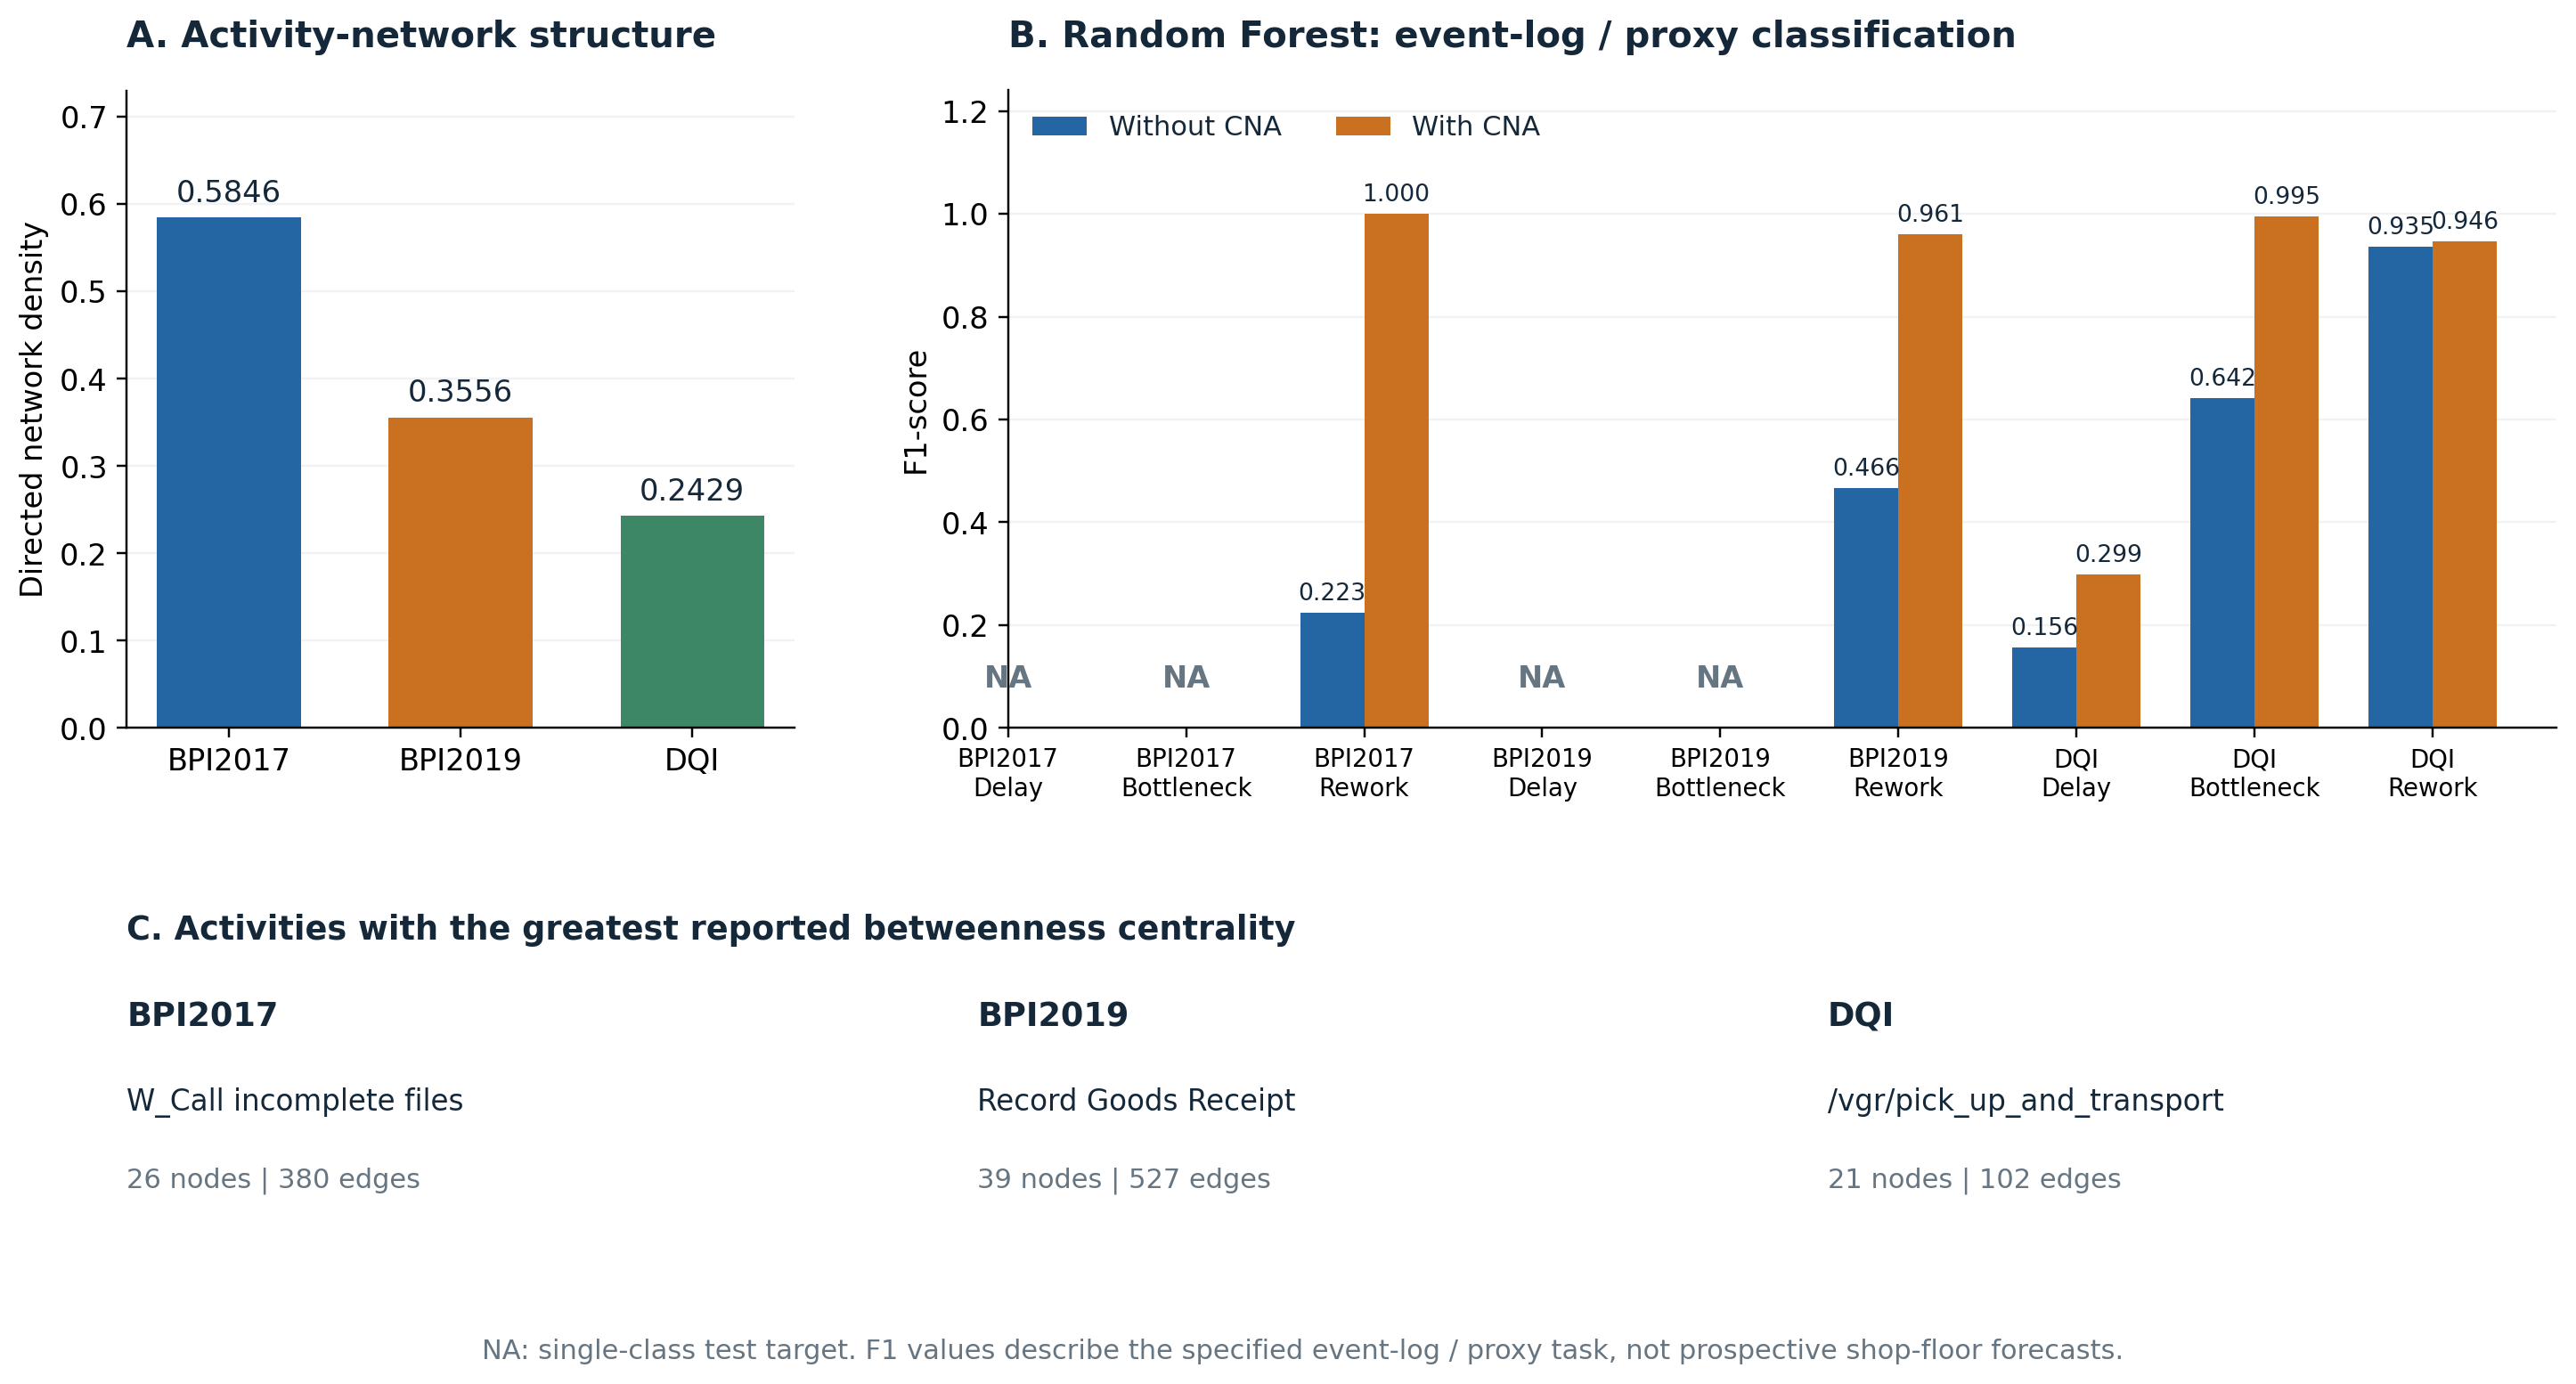
\includegraphics[width=\textwidth]{fig_real_datasets_experimental_results_dashboard}
\caption{Analytical results on BPI2017, BPI2019, and DQI. (A) Activity-network density. (B) Random Forest F1-scores with and without CNA features, using Table~\ref{tab:real_ml}; NA indicates a single-class test target. (C) Activities with the greatest reported betweenness centrality. Synthetic simulation results are presented separately. These classification results concern the event-log/proxy tasks described in the text.}
\label{fig:real_dashboard}
\end{figure*}

Table~\ref{tab:dataset_characteristics} summarizes the principal
characteristics of the evaluated event logs. BPI2019 represents the largest
dataset in terms of cases, activities, and organizational resources,
whereas DQI corresponds to a substantially smaller manufacturing process
characterized by pronounced quality-related issues. The considerable
differences in scale, process structure, and operational behavior make
these datasets appropriate for evaluating the robustness and
generalizability of the proposed framework.

\begin{table*}[t]
\caption{
Descriptive characteristics of the processed real-world event logs used for cross-domain analytical assessment. Counts refer to the analyzed subsets, not necessarily the complete public repositories.
}
\label{tab:dataset_characteristics}
\centering
\small
\begin{tabular}{lrrrrr}
\toprule
\textbf{Dataset} &
\textbf{Events} &
\textbf{Cases} &
\textbf{Activities} &
\textbf{Resources} &
\textbf{Observation Hours} \\
\midrule
BPI 2017 & 250,000 & 31,469 & 26 & 147 & 9,530.57 \\
BPI 2019 & 250,000 & 155,771 & 39 & 563 & 622,190.53 \\
Data Quality Issues & 8,607 & 271 & 21 & 15 & 5,977.72 \\
\bottomrule
\end{tabular}
\end{table*}

The descriptive process indicators reveal substantial differences in process
behavior across the evaluated datasets. The processed BPI files have reported processing-time fractions of approximately 28.1\% and 21.2\%. These fractions cannot be interpreted as validated value-added proportions because the preparation and timestamp lifecycle semantics differ by dataset. The BPI2019 start-time range includes 26 January 1948 through 18 January 2019; the 622,190.53-hour recorded span is therefore reported as a data characteristic, not a validated operating horizon for industrial throughput inference.

In contrast, the DQI dataset presents a Value-Added Ratio close to
100\%. This value should not be interpreted as evidence of near-perfect Lean
performance. Rather, in the supplied adapter the next-event gaps sum to case elapsed time, making the processing-time fraction approximately one by construction. The previous-event gaps are also recorded as waiting proxies, so these derived intervals must not be treated as independent measurements of value-adding service and queue time. This interpretation is particularly important
because the same dataset simultaneously exhibits a rework rate of
74.8\%, revealing substantial process instability that cannot be inferred
from conventional time-based Value Stream Mapping indicators alone.
Accordingly, this dataset illustrates the importance of complementing
traditional VSM analysis with quality-related, predictive, and structural
information.

Complex Network Analysis was subsequently applied to characterize structural
relationships among process activities. The resulting activity-network
properties are summarized in
Table~\ref{tab:network_metrics}.

\begin{table*}[t]
\caption{
Structural properties of the activity networks derived from the evaluated
real-world event logs. Reported activities correspond to the nodes with the
highest structural relevance according to betweenness centrality.
}
\label{tab:network_metrics}
\centering
\small
\begin{tabularx}{\textwidth}{lrrrrX}
\toprule
\textbf{Dataset} &
\textbf{Nodes} &
\textbf{Edges} &
\textbf{Density} &
\textbf{WCC} &
\textbf{Structurally Relevant Activity} \\
\midrule

BPI 2017 & 26 & 380 & 0.5846 & 1 & \texttt{W\_Call incomplete files} \\
BPI 2019 & 39 & 527 & 0.3556 & 1 & \texttt{Record Goods Receipt} \\
Data Quality Issues & 21 & 102 & 0.2429 & 1 & \texttt{/vgr/pick\_up\_and\_transport} \\
\bottomrule
\end{tabularx}
\end{table*}

As illustrated in Figure~\ref{fig:real_dashboard}A, BPI2017 exhibits the
highest activity-network density (0.5846), indicating comparatively strong
connectivity among process activities. BPI2019 presents an intermediate
density (0.3556), whereas DQI shows the sparsest network structure
(0.2429). The structurally relevant activities identified through
betweenness centrality analysis occupy strategically important positions
within the observed activity-flow networks and provide complementary
structural information beyond conventional flow-oriented Value Stream
Mapping indicators.

To evaluate the predictive contribution of structural information,
Machine Learning models were trained using two matched experimental
configurations: one employing only operational process features and another
augmenting the same feature set with Complex Network Analysis descriptors.
Following the temporal protocol described in
Section~\ref{subsec:training_protocol}, proxy-label thresholds were fitted on the training subset, and the stated
predictor exclusions were applied before evaluation on the temporally
held-out testing partition.

Table~\ref{tab:real_ml} summarizes the resulting predictive performance.

\begin{table*}[t]
\centering
\caption{
Temporally evaluated event-log classification on the real-world event logs.
F1-scores compare models using operational features only (No CNA) against
the same models augmented with CNA features.
}
\label{tab:real_ml}
\resizebox{\textwidth}{!}{%
\begin{tabular}{lllllll}
\toprule
Dataset & Target & Model & F1 (No CNA) & F1 (CNA) & $\Delta$F1 & Status \\
\midrule
BPI2017 & Delay & Random Forest & N/A & N/A & N/A & Single-class target \\
BPI2017 & Delay & XGBoost & N/A & N/A & N/A & Single-class target \\
BPI2017 & Bottleneck & Random Forest & N/A & N/A & N/A & Single-class target \\
BPI2017 & Bottleneck & XGBoost & N/A & N/A & N/A & Single-class target \\
BPI2017 & Rework & Random Forest & 0.2233 & 1.0000 & 0.7767 & Evaluable \\
BPI2017 & Rework & XGBoost & 0.0000 & 1.0000 & 1.0000 & Evaluable \\
BPI2019 & Delay & Random Forest & N/A & N/A & N/A & Single-class target \\
BPI2019 & Delay & XGBoost & N/A & N/A & N/A & Single-class target \\
BPI2019 & Bottleneck & Random Forest & N/A & N/A & N/A & Single-class target \\
BPI2019 & Bottleneck & XGBoost & N/A & N/A & N/A & Single-class target \\
BPI2019 & Rework & Random Forest & 0.4665 & 0.9608 & 0.4943 & Evaluable \\
BPI2019 & Rework & XGBoost & 0.0062 & 0.7453 & 0.7391 & Evaluable \\
Data Quality Issues & Delay & Random Forest & 0.1560 & 0.2989 & 0.1429 & Evaluable \\
Data Quality Issues & Delay & XGBoost & 0.0000 & 0.2210 & 0.2210 & Evaluable \\
Data Quality Issues & Bottleneck & Random Forest & 0.6421 & 0.9951 & 0.3530 & Evaluable \\
Data Quality Issues & Bottleneck & XGBoost & 0.0000 & 0.9975 & 0.9975 & Evaluable \\
Data Quality Issues & Rework & Random Forest & 0.9352 & 0.9463 & 0.0111 & Evaluable \\
Data Quality Issues & Rework & XGBoost & 0.9412 & 0.9508 & 0.0096 & Evaluable \\
\bottomrule
\end{tabular}%
}
\end{table*}

The table reports the corrected-code execution with mixed-format UTC timestamp parsing and stable temporal row ordering. The original parser silently rejected 467 otherwise valid BPI2017 rows and six otherwise valid DQI rows; all rows are retained by the corrected parser. Stable ordering also makes the tie convention explicit. Original-code reproductions are retained separately in the audit materials. For BPI2017 they reproduce the reported RF change from 0.2243 to 1.0000; the corrected run yields 0.2233 to 1.0000.

The BPI delay and operational-bottleneck test tasks remain single class under the stated proxy definitions and are reported as unavailable. In particular, waiting-time proxies are constant zero in both prepared BPI files, making the upper-percentile waiting rule uninformative. This is a limitation of the prepared representation rather than evidence that no real delays or bottlenecks occurred.

In BPI2017, all positive prepared rework labels occur at \texttt{O\_Returned}, and every occurrence of that activity is positive. On the corrected 37,500-event test set, an activity-majority rule fitted only on training rows attains F1 = 1.0000, as do the activity-one-hot and training-only network classifiers. The perfect score is thus explained by a deterministic activity--label association in the prepared data; a graph descriptor can serve as an activity signature. It is not evidence that network analysis anticipates future rework or outperforms an activity-only diagnostic baseline.

In BPI2019, positive labels identify a subset of change-related activities. The training-derived activity-majority and activity-only classifiers also attain F1 = 1.0000 on the audited test set. The network-augmented classifiers therefore cannot establish added predictive value beyond the available activity identity. Differences from operational-only models quantify a representation change, not a uniquely structural or causal improvement.

The DQI label represents repeated within-case activity occurrences in the supplied preparation. Its current-event timing and repetition semantics differ from the activity-defined BPI labels. The corrected DQI F1 values are retained in Table~\ref{tab:real_ml}, with activity-baseline results in Table~\ref{tab:real_activity_audit}. Small differences from the original manuscript are documented in the reproduction materials rather than hidden by retaining obsolete rounded values.

\begin{table*}[t]
\caption{Executed activity-baseline comparison for the rework/repetition label. Real-log rows use mixed-format timestamp parsing, stable temporal ordering, and balanced Random Forest class weights; the synthetic RF is unweighted, matching its original classifier. All rules and graph descriptors use training rows only.}
\label{tab:real_activity_audit}
\centering\small
\begin{tabular}{lrrrrrr}
\toprule
Dataset & Test events & Positives & Operational RF & + CNA RF & Activity rule & Activity RF\\
\midrule
Synthetic & 1,280 & 21 & 0.2500 & 1.0000 & 1.0000 & 1.0000 \\
BPI2017 & 37,500 & 846 & 0.2233 & 1.0000 & 1.0000 & 1.0000 \\
BPI2019 & 37,500 & 1,276 & 0.4665 & 0.9608 & 1.0000 & 1.0000 \\
DQI & 1,292 & 948 & 0.9352 & 0.9463 & 0.8464 & 0.4817 \\
\bottomrule
\end{tabular}
\end{table*}

The corrected row split shares seven BPI2017 cases and 2,424 BPI2019 cases between training and test; DQI shares none between those partitions. These counts make the evaluation explicitly event-held-out rather than a claim of unseen-case generalization. The metadata and saved predictions identify the observation windows and class counts.

The real-log code constructs its activity graph exclusively from training rows, and unseen activities receive zero centralities. That control is implemented and is sufficient to rule out direct construction of those graph features from held-out rows in this script. It does not establish a future-event forecasting design: current-event durations can depend on later completion information, and cases overlap the row partitions. The revised interpretation is diagnostic classification of the defined prepared labels.

\subsection{Cumulative Scenario Comparison}
\label{subsec:ablation_results}

The scenario comparison evaluates the predefined factor sets G0--G5. Figure~\ref{fig:ablation_improvement} and Table~\ref{tab:ablation_results} summarize the resulting model indicators. These are cumulative scenario assumptions rather than observed module-addition effects.

\begin{figure*}[t]
\centering
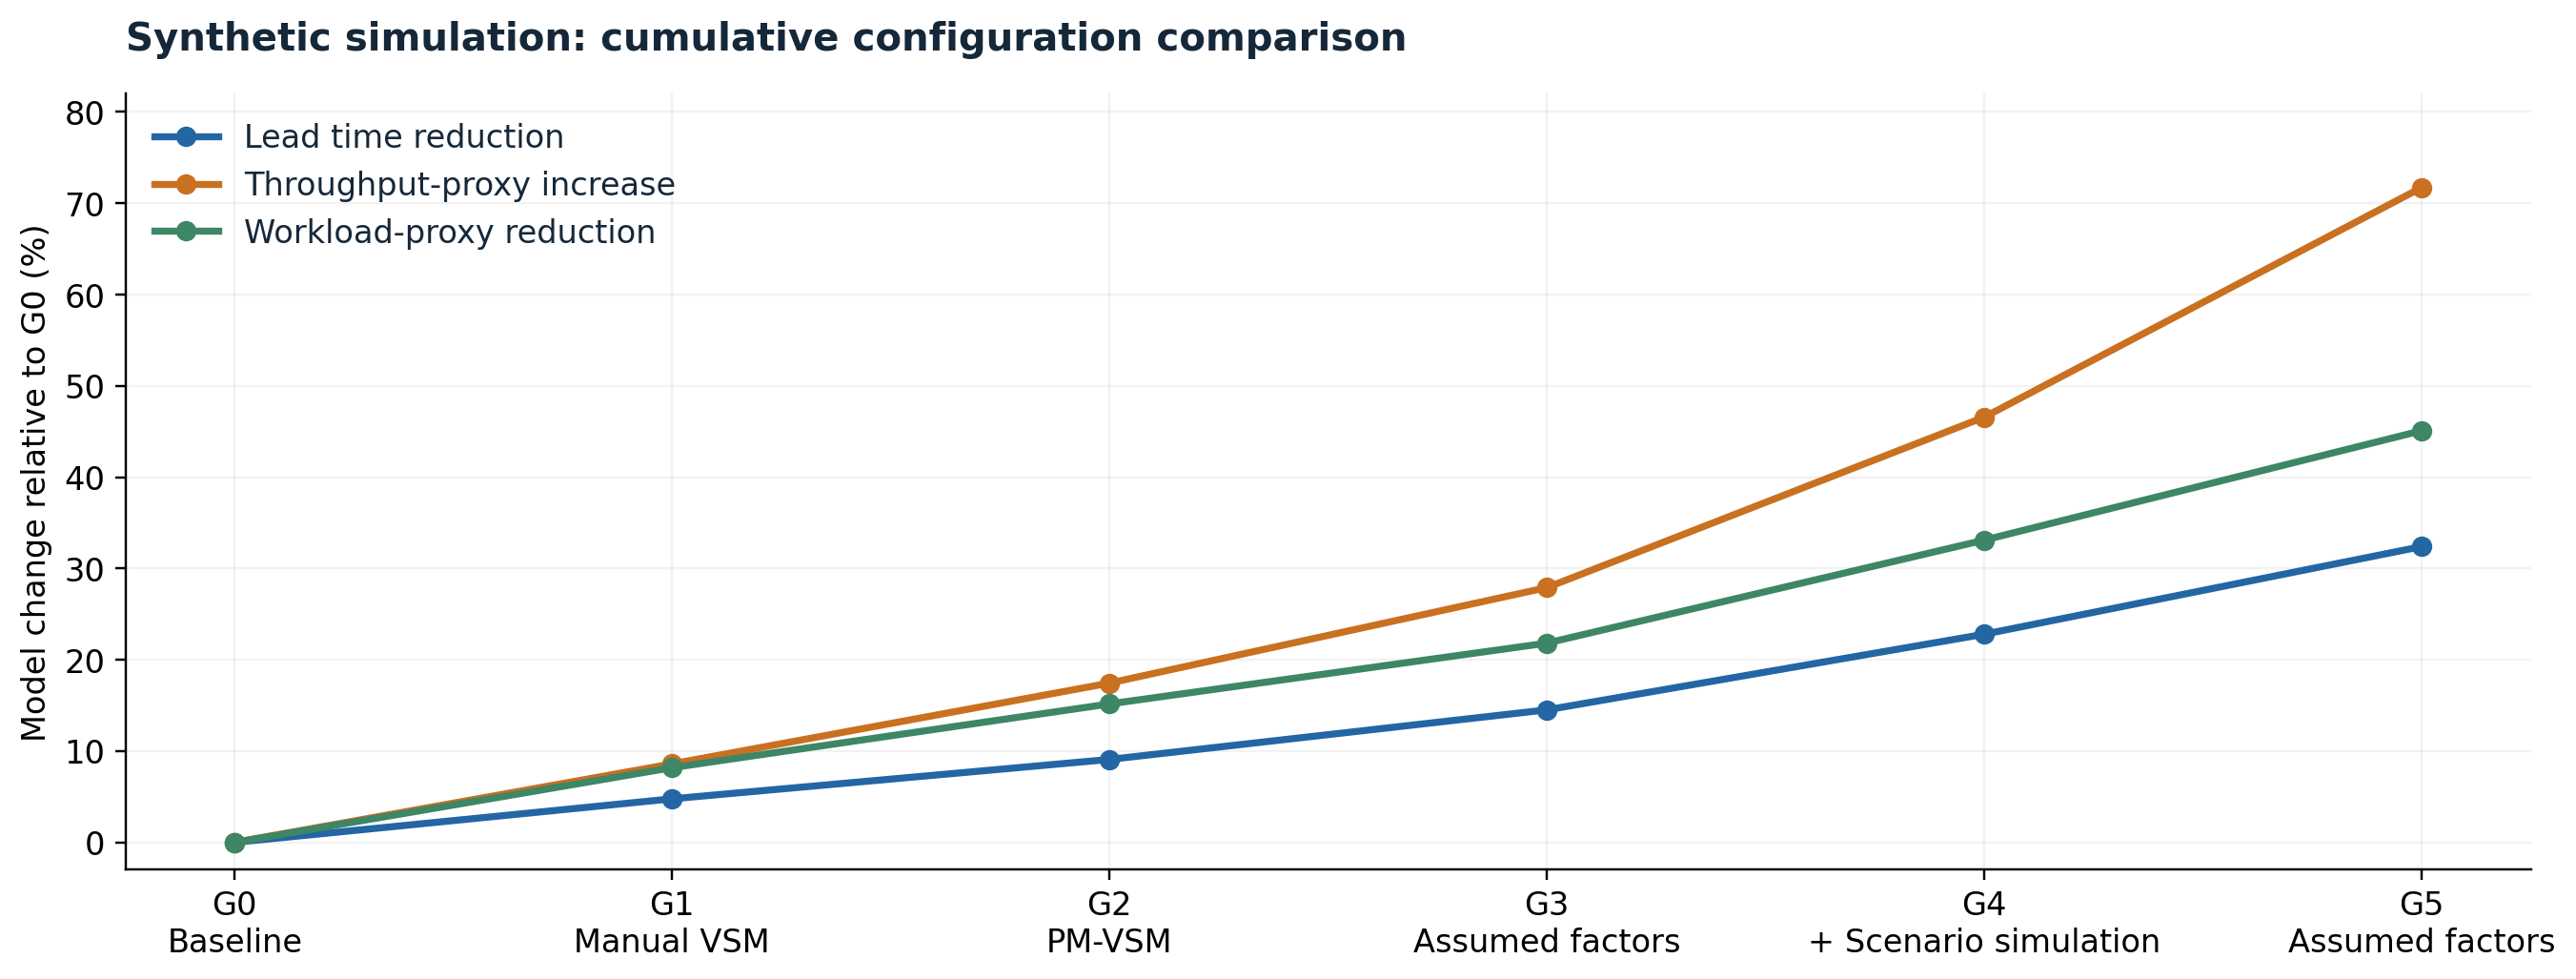
\includegraphics[width=\textwidth]{fig_6_ablation_improvement}
\caption{Simulated relative KPI changes across the cumulative configurations. Values follow Table~\ref{tab:ablation_results}; MCS denotes offline Monte Carlo simulation, and the G4 throughput increase is 46.6\%. These are synthetic scenario outcomes rather than measurements after physical implementation.}
\label{fig:ablation_improvement}
\end{figure*}

\begin{table*}[t]
\centering
\caption{
Relative KPI changes across cumulative configurations in the synthetic manufacturing simulation.
}
\label{tab:ablation_results}
\begin{tabular}{lrrr}
\toprule
\textbf{Configuration} &
\textbf{LT reduction} &
\textbf{TH gain} &
\textbf{WIP reduction} \\
& \textbf{(\%)} & \textbf{(\%)} & \textbf{(\%)} \\
\midrule
G0 -- Baseline & 0.0 & 0.0 & 0.0 \\
G1 -- Manual VSM & 4.8 & 8.6 & 8.2 \\
G2 -- PM-VSM & 9.1 & 17.4 & 15.2 \\
G3 -- PM-VSM + XAI & 14.5 & 27.9 & 21.8 \\
G4 -- PM-VSM + XAI + MCS & 22.8 & 46.6 & 33.1 \\
G5 -- Complete framework & 32.4 & 71.7 & 45.1 \\
\bottomrule
\end{tabular}
\end{table*}

The G5 factor set produces the largest favorable changes among the six scenarios. Relative to G0, sampled lead time is 32.40\% lower, the workload proxy is 45.09\% lower, station defect proportion is 27.63\% lower, order rework proportion is 45.52\% lower, and the calendar-based throughput proxy is 71.73\% higher. The code-level reproduction confirms these numbers; it does not establish an analytical or industrial mechanism that would generate the assumed factor settings.

Consequently, the scenario comparison demonstrates how the specified sampler responds to assumptions about redesign. It cannot quantify the benefit of adding PM, XAI, or CNA. Such attribution would require interventions generated through reproducible analytical rules and comparison under common operational constraints, or deployment evidence.

\subsection{Statistical Validation of the Simulation Results}
\label{subsec:statistical_results}

Re-execution of the original scenario sampler reproduces all five headline percentages to the precision reported. Because scenarios reuse each replication's initial seed, the audit applies the blocked procedure described in Section~\ref{subsec:statistical_validation}. Table~\ref{tab:paired_statistics} reports G5--G0 relative changes, paired-bootstrap intervals, and Holm-adjusted baseline-comparison p-values.

\begin{table*}[t]
\caption{Executed seed-blocked G5--G0 scenario comparison. Relative-change intervals use paired replication-block bootstrap resampling. P-values are adjusted across five baseline comparisons within each KPI. These are conditional model outcomes, not causal effects of analytical modules.}
\label{tab:paired_statistics}
\centering\small
\begin{tabular}{lrrr}
\toprule
Indicator & Change (\%) & Bootstrap 95\% interval (\%) & Adjusted p\\
\midrule
Lead time reduction & 32.40 & [32.26, 32.54] & $ 9.31 \times 10^{-9} $ \\
Workload-proxy reduction & 45.09 & [44.66, 45.53] & $ 9.31 \times 10^{-9} $ \\
Defect-rate reduction & 27.63 & [25.45, 29.83] & $ 8.63 \times 10^{-6} $ \\
Rework-rate reduction & 45.52 & [40.72, 50.00] & $ 8.64 \times 10^{-6} $ \\
Throughput-proxy increase & 71.73 & [71.72, 71.74] & $ 9.31 \times 10^{-9} $ \\
\bottomrule
\end{tabular}
\end{table*}

All five G5--G0 comparisons remain significant within this sampler. This establishes stochastic differences between scenarios with different assumed factors. It does not validate physical throughput or inventory, estimate the contribution of a software module, or establish that model diagnosis caused the factor settings. The audit therefore supports H1 only as a within-model scenario comparison; H2 requires interpretation against activity-only baselines, and the broader integrated deployment proposition remains to be established.

\section{Discussion}
\label{sec:discussion}

The contribution is a traceable connection between current-state reconstruction, structural and model-assisted diagnosis, candidate intervention definition, offline assessment, and future-state representation. Rather than treating the analytical technologies as independent endpoints, the workflow organizes their outputs around decisions about process redesign. Model explanations and centrality indicators identify associations and structurally important elements; they do not establish causal intervention effects on their own.

The operational and analytical results have distinct scopes. Code inspection shows that the scenario sampler does not load the fitted ML models, explanations, or network metrics to determine its factors. Consequently, the six named configurations are assumed intervention scenarios rather than an executed component-ablation experiment. The complete G0--G5 comparison concerns a synthetic manufacturing simulation. The reductions of 32.40\% in lead time, 45.09\% in WIP, 27.63\% in defect rate, and 45.52\% in rework rate, with a throughput increase of 71.73\%, are simulated estimates conditional on the modeled system and intervention settings. The within-model statistical comparison addresses stochastic replication variability. It does not establish that these exact magnitudes transfer to physical production or that the simulator reproduces every industrial exception.

The numerical design compares predefined intervention factors associated conceptually with progressively enriched workflows. It does not isolate causal effects of individual modules, nor show that adding software alone improves production. A factorial design, component-removal comparison, and intervention-cost analysis would help separate analytical benefits from differences in the operational changes selected under each configuration.

The BPI benchmarks extend the analytical assessment to financial administration and procurement. An active-case count can provide an administrative workload analogue to WIP, but it is not physical inventory. Similarly, repeated administrative activities are repetition proxies unless corrective intent is confirmed, and measured processing time is not automatically value added. The domain-specific interpretations in Table~\ref{tab:domain_adaptation} are necessary for transfer of the workflow and prevent administrative classification scores from being presented as manufacturing validation.

The synthetic and real-log audits show that an activity-only rule suffices for perfect synthetic and BPI rework-label classification. Original BPI2017 results are reproduced, and the corrected reader retains valid timestamps previously dropped. The F1 = 1.0000 BPI2017 result is explained by the activity-defined target and a training-only activity signature. This control rules out the need for held-out graph construction to attain the perfect diagnostic result, but it does not establish a prospective forecasting capability. The near-perfect DQI operational-proxy classification has a related activity-level construct limitation. The results therefore support discussion of retrospective diagnostic separability rather than a claim of perfect prediction of future rework or physical bottlenecks. Prospective validation would require explicit decision timestamps and outcome horizons, prefix-only features, causal graph construction, and case-boundary handling.

\subsection{Resilience and Sustainability Implications}
\label{subsec:resilience_sustainability}

Industrial resilience concerns the capacity to sustain and recover operations under disruption. The workflow could support this objective by evaluating resource failures, demand surges, routing exceptions, and incomplete records as explicit intervention scenarios. Relevant outcomes would include service-level degradation, backlog accumulation, recovery time, and performance over disruption severity. The present nominal scenario comparison does not measure recovery or demonstrate resilience gains; these are concrete directions for extending the evaluation.

Sustainability-integrated VSM provides a relevant framework for connecting operational process analysis with environmental information \cite{HorsthoferRauch2024SustainabilityVSM}. Reduced rework or waiting may motivate investigation of resource savings, but lower operational waste does not by itself demonstrate lower energy use or emissions. Increased throughput and added capacity can introduce trade-offs. A sustainability extension should therefore measure energy per conforming unit, material loss, water use where relevant, and emissions under stated system boundaries, together with worker workload and safety. These indicators would allow explicit comparison with cost, lead time, and quality rather than assuming that operational gains automatically imply environmental or social improvement.

\subsection{Deployment and Evidence Boundaries}

A manufacturing deployment should establish the process boundary, timestamp semantics, resource constraints, and independently observed quality criteria. Simulation parameters should be estimated from an initial operating period and checked against a separate period before candidate interventions are assessed. Physical implementation followed by longitudinal measurements would then evaluate whether modeled benefits persist under changing demand, product mix, equipment failure, and exceptional routing.

The proposed closed loop links diagnosis, intervention definition, simulation, and VSD. The numerical implementation evaluates diagnostic components and separately specified scenarios; it does not demonstrate an automatic causal path from a diagnostic output to a selected intervention or a validated redesigned plant. Physical implementation and a subsequent operating period were not evaluated. The supplied scripts implement an activity DFG and classification comparisons; resource/value-flow networks, SHAP explanations, conformance checking, and a shared-resource simulation remain proposed capabilities. A synchronized DT architecture could extend the workflow \cite{GrievesVickers2017,Aheleroff2021DTaaS}, but live connectivity and recurrent automatic recalibration are not capabilities established by this study.

\section{Conclusions and Future Work}
\label{sec:conclusions}

This paper presents a data-driven VSM/VSD workflow linking operational event logs, current-state reconstruction, structural and model-assisted diagnosis, offline scenario analysis, and future-state design. Its contribution is methodological integration and traceability across decision-support stages rather than a new prediction algorithm or a demonstrated live DT deployment.

In the predefined Monte Carlo scenario comparison, G5 yielded reductions of 32.40\% in lead time, 45.09\% in WIP, 27.63\% in defect rate, and 45.52\% in rework rate, with a throughput increase of 71.73\% relative to G0. These are responses to assumed scenario factors, including model-defined workload and calendar-based throughput proxies, not improvements measured after implementation on a shop floor. The administrative benchmarks assess cross-domain analytical components, and their classification results must be interpreted according to the event-log and proxy-label definitions.

Future work should evaluate prospectively available features and independently observed outcomes, characterize sensitivity to process and data-quality disruptions, and assess implemented interventions in a physical manufacturing setting. Cost-aware redesign, sustainability indicators, disruption/recovery analysis, and validated physical--digital synchronization provide further extensions of the workflow.

\section*{Statements and Declarations}

\subsection*{Competing Interests}
The authors declare that they have no competing interests.

\subsection*{Funding}
The authors received no specific funding for this work.

\subsection*{Author Contributions}
Edwin Montes-Orozco: Conceptualization, Methodology, Software, Formal Analysis, Writing -- Original Draft, Visualization.
Mariam Dopslaf: Conceptualization, Supervision, Validation, Writing -- Review \& Editing.
Roman Anselmo Mora-Guti\'errez: Validation, Formal Analysis, Writing -- Review \& Editing.
Sergio Gerardo de-los-Cobos-Silva: Methodology, Validation, Writing -- Review \& Editing.
Eric Alfredo Rinc\'on-Garc\'ia: Formal Analysis, Validation, Writing -- Review \& Editing.
Pedro Lara-Vel\'azquez: Validation, Supervision, Writing -- Review \& Editing.
Miguel \'Angel Guti\'errez-Andrade: Validation, Supervision, Writing -- Review \& Editing.

\subsection*{Data Availability}
The synthetic manufacturing event log, route parameters, original analysis scripts, and reproducibility materials for the revised analyses are publicly available at \url{https://github.com/emontes200892/data-driven-vsm-vsd-framework}. The revision materials are organized in \texttt{revision\_2026\_11\_02/}, with original and corrected implementations and outputs kept separate.

This directory contains the exact prepared CSVs evaluated in the revised analyses, their SHA-256 hashes, the synthetic generator and inputs, original and corrected scripts, held-out audit predictions, scenario replications, and statistical outputs. The materials are accessible through the repository without a separate supplementary ZIP upload. The public BPI benchmark descriptions and dataset records are cited in the references. The prepared BPI label associations and timestamp parsing are audited explicitly. The generic XES adapter supplied with the study is not asserted to be the preparation provenance of the BPI files; raw-source transformation provenance remains an external-validity limitation.

\subsection*{Ethics Approval and Consent to Participate}
Not applicable. No new human-subject intervention or animal experiment was conducted;
the study uses synthetic manufacturing data and publicly released
process-event benchmarks.

\subsection*{Consent for Publication}
Not applicable.

\bibliography{references_corrected}

\end{document}
